\chapter{Calibrazione Energetica del Rivelatore}
\label{ch:calibrazione}

La calibrazione energetica costituisce uno dei passaggi cardine nell'analisi dei dati di un esperimento di fisica delle particelle. Nell'ambito di CRESST, essa consiste nel determinare la relazione che converte l'ampiezza degli impulsi, misurata in Volt tramite l'\textit{Optimum Filter Pulse Height}, nella corrispondente energia rilasciata nel cristallo, espressa in $\text{keV}$. 

Stabilire con accuratezza questa corrispondenza è indispensabile per due ragioni fondamentali: da un lato permette di quantificare la reale soglia energetica del rivelatore ($E_{\text{th}}$) a partire dalla soglia in \text{mV} ($V_{\text{th}}$) determinata nel capitolo precedente, che definisce la sensibilità dell'apparato a rilasci microscopici, dall'altro consente di ricostruire correttamente l'energia depositata da eventuali eventi candidati di materia oscura.

Operativamente, la calibrazione viene effettuata esponendo il rivelatore a sorgenti radioattive che emettono fotoni o particelle di energia nota. In questo modo è possibile tracciare una curva di risposta sperimentale ($\text{V} \rightarrow \text{keV}$). L'energia di qualsiasi evento successivo potrà quindi essere determinata univocamente interpolando l'ampiezza ricostruita lungo tale curva.

\section{Strategie di Calibrazione: Limiti del $^{55}\text{Fe}$ e Sorgente di $^{57}\text{Co}$}
\label{sec:strategie_calibrazione}

Tra i candidati primari impiegati per la calibrazione nei rivelatori criogenici spicca il $^{55}\text{Fe}$. Questo atomo decade per cattura elettronica emettendo raggi X caratteristici del manganese, dominati dal doppietto $K_\alpha$ a $5.89\,\text{keV}$ e $K_\beta$ a $6.49\,\text{keV}$. La vicinanza di queste righe alla regione del keV è ideale per vincolare la risposta sperimentale a bassa energia; tuttavia, il loro impiego diretto nei run scientifici standard presenta un limite operativo.

Per schermare gli esperimenti di fisica degli eventi rari dal fondo ambientale e dalla radioattività naturale, l'apparato sperimentale è alloggiato all'interno di una serie concentrica di schermi, come illustrato nel Paragrafo \ref{subsec:criostato}. A causa dell'energia ridotta, i fotoni da circa $6\,\text{keV}$ verrebbero interamente assorbiti dalle pareti esterne prima di raggiungere il cristallo. L'unica soluzione praticabile consiste dunque nel posizionare la sorgente di $^{55}\text{Fe}$ direttamente all'interno dell'ultimo stadio del criostato, nelle immediate vicinanze del cristallo. 

Tale configurazione comporta tuttavia una complicazione fondamentale: per rimuovere il campione al termine della fase di calibrazione è indispensabile riscaldare il criostato fino a temperatura ambiente per poi eseguire un nuovo ciclo di raffreddamento. Questo processo compromette la validità della calibrazione appena effettuata per due motivi:
\begin{enumerate}
    \item Ogni ciclo termico altera il TES, modificandone lievemente la curva di transizione $R(T)$ e obbligando a identificare un punto di lavoro differente;
    \item La nuova sequenza di raffreddamento ripristina gli stress reticolari nel cristallo e nei supporti di sostegno, i cui rilassamenti causano il cosiddetto \textit{Low Energy Excess} (LEE), un fondo a bassa energia che decade esponenzialmente nel tempo.
\end{enumerate}
Lasciare invece la sorgente costantemente montata all'interno introdurrebbe un fondo radioattivo irriducibile, dovuto al continuo decadimento del $^{55}\text{Fe}$, incompatibile con la ricerca di eventi rari.
Per superare questo vincolo si rende necessario l'impiego di una sorgente $\gamma$ a più alta energia, in grado di penetrare gli schermi dall'esterno del criostato per poi essere rimossa agevolmente senza interrompere il regime criogenico. La scelta effettuata e analizzata in questa tesi è ricaduta sul $^{57}\text{Co}$, che decade principalmente tramite emissioni a $122.06\,\text{keV}$ e $136.47\,\text{keV}$. Questi fotoni possiedono una penetrazione sufficiente ad attraversare gli schermi e interagire per effetto fotoelettrico o scattering Compton nel cristallo, permettendo la rimozione immediata della sorgente prima di avviare la presa dati di fondo.

L'adozione del Cobalto solleva però un quesito cruciale: CRESST opera nella regione sub-keV per massimizzare la sensibilità a particelle di materia oscura di massa leggera, mentre il $^{57}\text{Co}$ deposita energie superiori ai $100\,\text{keV}$. È lecito assumere che la calibrazione definita a energie così elevate rimanga valida anche nella zona di interesse, ovvero a due ordini di grandezza inferiori?

Per rispondere a questa domanda è stato condotto un run dedicato esponendo simultaneamente il rivelatore a entrambe le sorgenti ($^{57}\text{Co}$ all'esterno e $^{55}\text{Fe}$ all'interno). L'obiettivo primario di questa analisi consiste nel determinare la curva di calibrazione a partire dai picchi ad alta energia del Cobalto per poi verificare se, prolungata verso il fondo scala, intercetti con precisione le righe del Ferro, validando sperimentalmente l'affidabilità dell'estrapolazione a bassa soglia.

\section{Ricostruzione dei Segnali Saturi e Studio della Linearità}
\label{sec:ricostruzione_saturi}

Per caratterizzare la linearità della catena di lettura e la risposta dinamica del sensore, sono stati preliminarmente analizzati gli impulsi di test artificiali (\textit{testpulses}). Come introdotto nel Paragrafo~\ref{sec:struttura_dati} (e illustrato in Figura~\ref{fig:PulsesComparison}b), tali segnali vengono generati iniettando impulsi di corrente di ampiezza nota su una resistenza di riscaldamento (\textit{heater}) evaporata direttamente sul cristallo assorbitore. 

In Figura~\ref{fig:TestPulse_non_ricostruiti} è riportata la risposta del calorimetro in funzione della tensione iniettata sull'heater. La popolazione di testpulse analizzata è stata presa attraverso una scrematura a $3\sigma$ standard dal centro e iterata più volte fino a stabilizzazione dell'algoritmo. 

L'andamento evidenzia in modo marcato la deviazione dal regime lineare. La retta visualizzata interpola i primi quattro livelli di testpulse, la cui ampiezza ricostruita dall'\textit{Optimum Filter} risulta inferiore a circa $1\,\text{V}$: in questo intervallo la risposta del rivelatore è ancora lineare. Al crescere dell'energia iniettata, tuttavia, i punti sperimentali mostrano una netta curvatura verso l'alto: l'incremento di temperatura spinge la curva di transizione del TES verso l'estremità superiore $R(T)$, determinando la saturazione del segnale e limitando l'ampiezza massima misurabile. 

\begin{figure}[htbp]
    \centering
    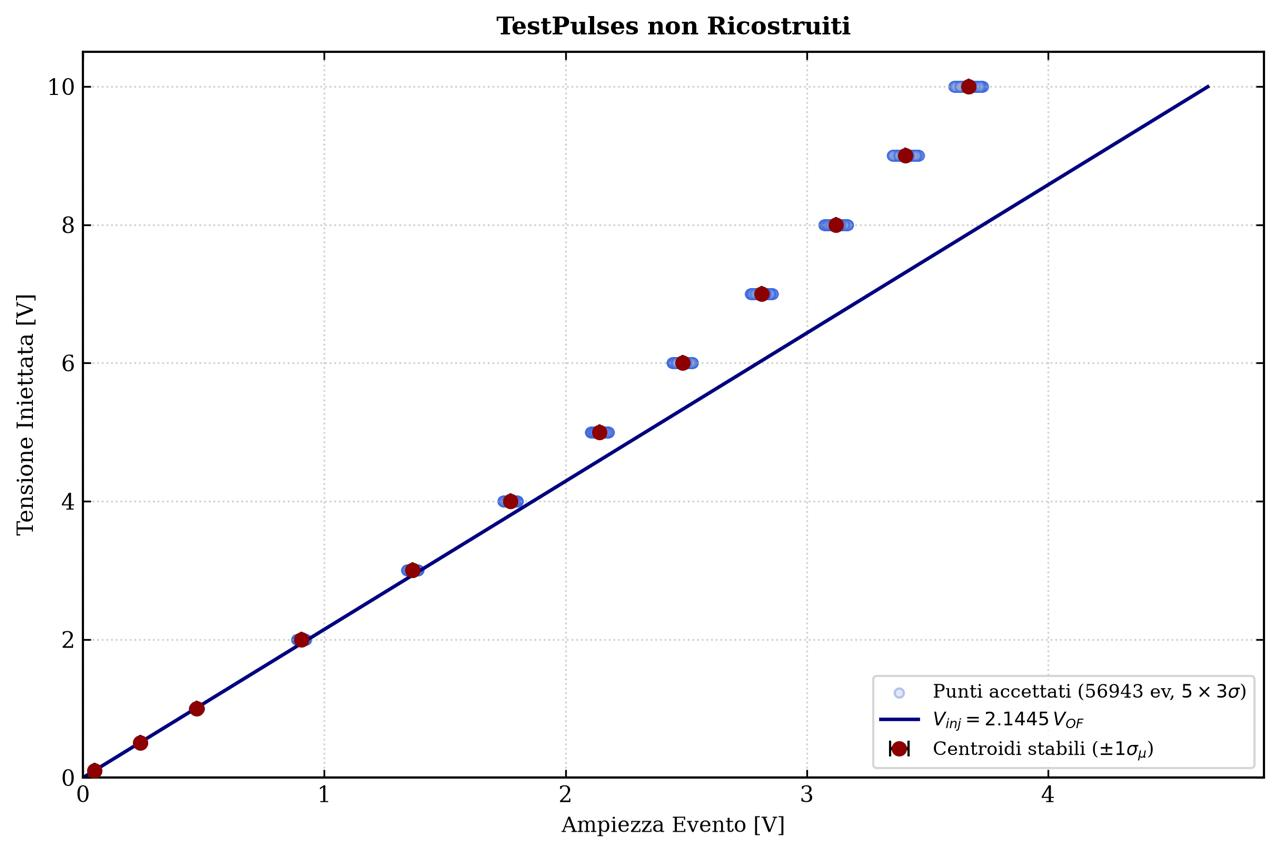
\includegraphics[width=0.8\textwidth]{figures/TestPulses_non_ricostruiti.jpeg}
    \caption{Risposta del rivelatore in funzione dei testpulses iniettati. Sull'asse delle ordinate è riportata la tensione applicata all'heater (a gradini discreti di ampiezza nota), mentre sull'asse delle ascisse figura l'ampiezza stimata tramite il filtraggio convenzionale con \textit{Optimum Filter} (\ref{sec:teoria_OF}). La linea continua rappresenta l'estrapolazione della risposta lineare determinata sui primi quattro punti.}
    \label{fig:TestPulse_non_ricostruiti}
\end{figure}

Poiché i fotoni di calibrazione emessi dal $^{57}\text{Co}$ ($122\,\text{keV}$ e $136\,\text{keV}$) rilasciano un'energia che ricade ampiamente nella regione di saturazione del TES, l'impiego dell'Optimum Filter standard produrrebbe una severa compressione della scala energetica. Si rende pertanto indispensabile un algoritmo dedicato alla ricostruzione dell'ampiezza reale degli eventi saturi.

\subsection{Ricostruzione del picco con CAIT}
\label{subsec:Ricostruzione_picco}

La ricostruzione dell'ampiezza non saturata è stata condotta mediante gli algoritmi implementati nel pacchetto di analisi \texttt{cait} (\textit{CRESST Analysis with Interactive Tools}). 

Il principio su cui si fonda l'algoritmo discende dal modello descritto dall'Equazione~\eqref{eq:segnale_modello}: nell'ipotesi che la dinamica termica di rilassamento del calorimetro non subisca alterazioni strutturali e che la non-linearità sia imputabile primariamente alla saturazione della transizione del TES, la forma d'onda del segnale ideale può essere descritta scalando il template unitario di riferimento $s(t - t_0)$ per un'ampiezza libera $A$:
\begin{equation}
    v_{\text{modello}}(t) = A \cdot s(t - t_0).
\end{equation}
L'obiettivo risiede dunque nello stimare il parametro $A$ anche quando il picco dell'impulso risulta troncato o distorto dalla saturazione dell'elettronica e del sensore.

La distorsione non si manifesta unicamente nel plateau orizzontale alla massima tensione, ma contamina anche la fase iniziale della discesa, dove il film superconduttore permane in uno stato parzialmente resistivo fuori dalla regione di linearità. Per preservare l'affidabilità della stima è necessario definire un valore di soglia massima di tensione, denominato \textit{truncation limit} (TL). La scelta di questo parametro riflette un compromesso ottimale:
\begin{itemize}
    \item un valore di TL eccessivamente elevato includerebbe nel fit campioni temporali situati nella zona di forte non-linearità del TES, distorcendo sistematicamente la stima dell'ampiezza $A$;
    \item un valore di TL troppo conservativo (eccessivamente basso) scarterebbe una porzione rilevante della traccia, lasciando un numero insufficiente di samples accettati e aumentando l'errore sul picco dell'evento ricostruito
\end{itemize}

Per identificare oggettivamente la soglia ottimale è stato studiato l'andamento dell'RMS del fit su tutti gli eventi disponibili, variando progressivamente l'ampiezza del segnale. Come evidenziato in Figura~\ref{fig:Scelta_TL}, l'RMS si mantiene piatto e costante a bassi voltaggi, per poi esibire una rapida crescita in corrispondenza di ampiezze superiori a circa $1.3\,\text{V}$, segnalando l'insorgenza della distorsione di forma. In via conservativa, il \textit{truncation limit} è stato quindi fissato al valore di $1.0\,\text{V}$.

\begin{figure}[htbp]
    \centering
    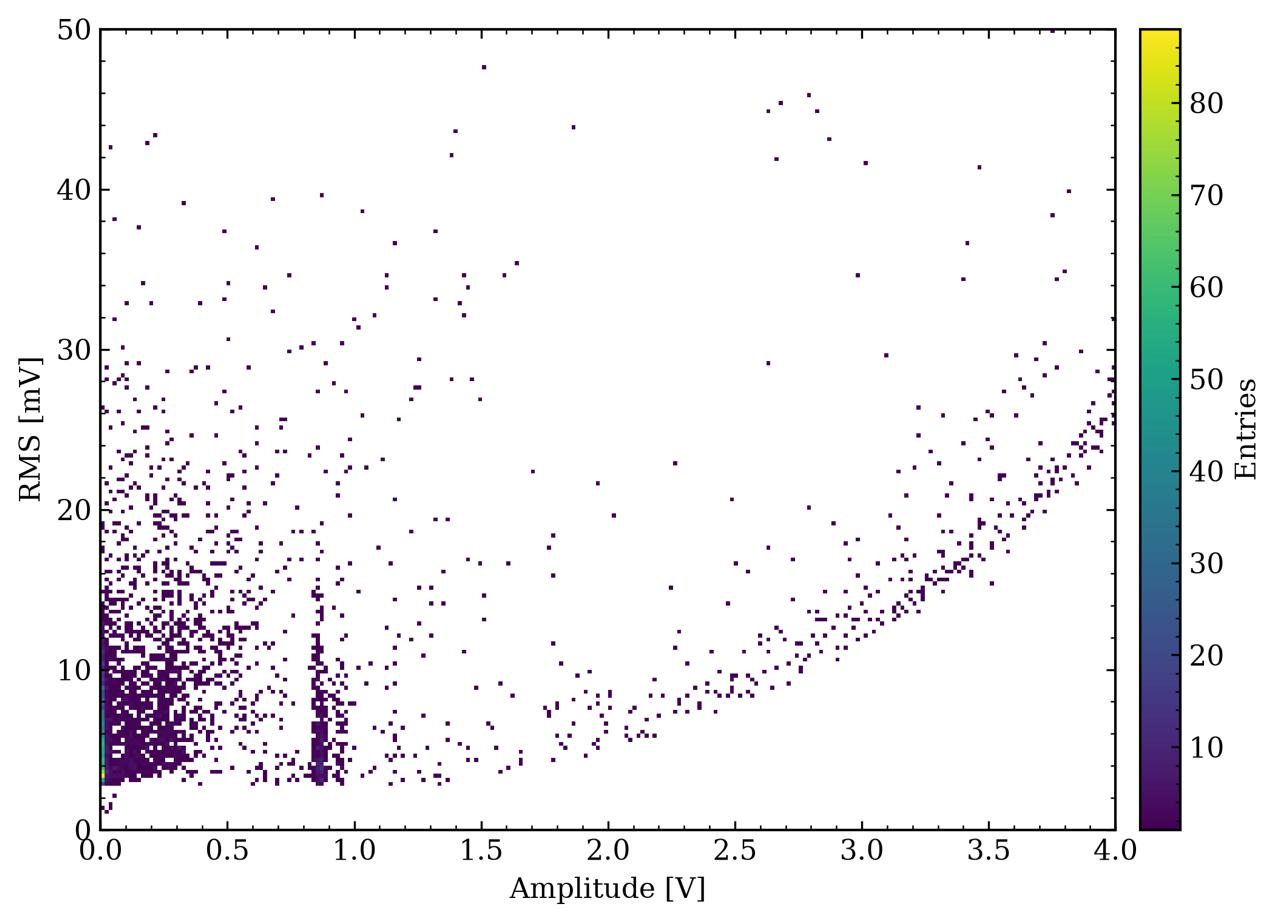
\includegraphics[width=0.7\textwidth]{figures/Analisi_TL.jpeg}
    \caption{Andamento del residuo RMS del fit in funzione dell'ampiezza dell'impulso. A partire da circa $1.3\,\text{V}$ si osserva un graduale incremento dell'RMS, indice dell'incapacità del modello di descrivere i campioni soggetti a saturazione resistiva.}
    \label{fig:Scelta_TL}
\end{figure}

Fissato il TL a $1.0\,\text{V}$, l'algoritmo di \texttt{cait} esclude tutti i punti della finestra di acquisizione aventi ampiezza superiore a tale soglia, poiché presentano effetti di saturazione. Sul sottoinsieme di punti rimanenti (comprendente la linea di base pre-trigger, il fronte di salita iniziale e la coda asintotica di rilassamento termico), viene eseguita una minimizzazione dei minimi quadrati per estrarre il fattore di scala ottimale $A$. Un esempio rappresentativo di evento saturo ricostruito con questo approccio è mostrato in Figura~\ref{fig:Impulso_ricostruito}.

\begin{figure}[htbp]
    \centering
    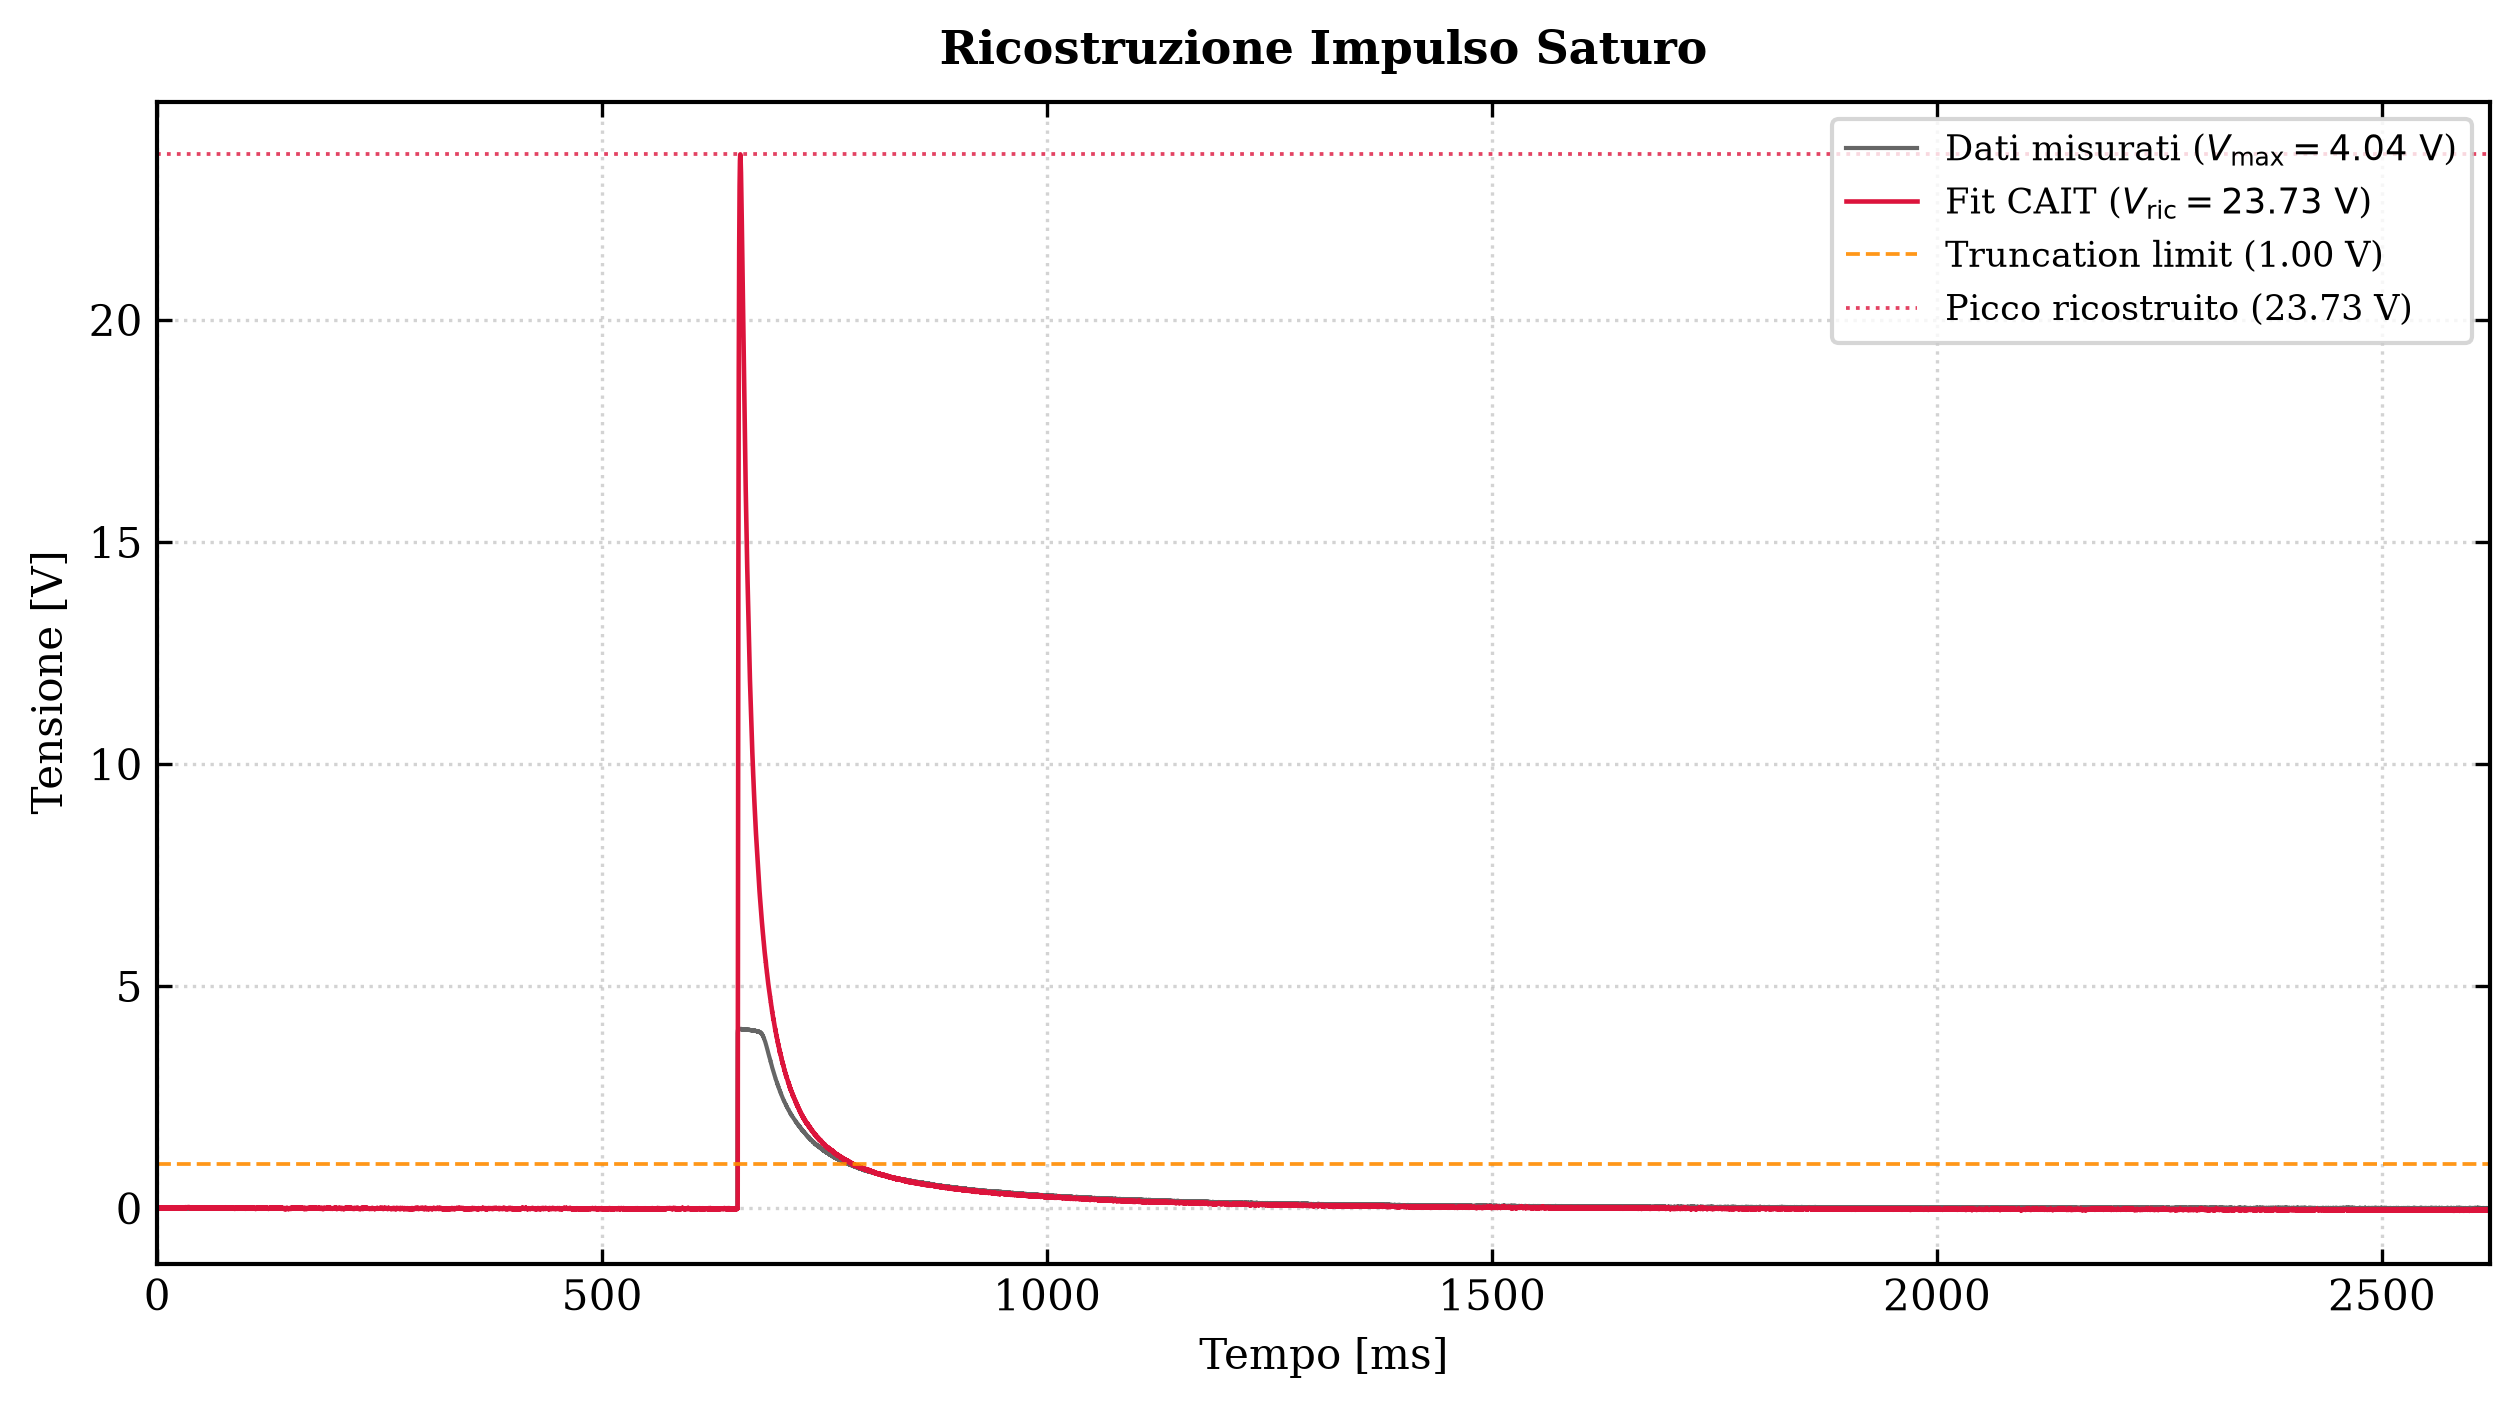
\includegraphics[width=0.8\textwidth]{figures/Impulso_ricostruito.png}
    \caption{Esempio di ricostruzione di un impulso saturo mediante l'algoritmo di troncatura di \texttt{cait}. La traccia sperimentale grezza (in nero) presenta una netta saturazione a circa $4\,\text{V}$. I campioni situati al di sopra del \textit{truncation limit} di $1\,\text{V}$ (linea orizzontale arancione) non vengono considerati dall'algoritmo. La curva rossa rappresenta il template ottimale riscalato per il fattore di ampiezza stimato ($A = 23.73\,\text{V}$), riproducendo l'escursione ideale che l'impulso avrebbe descritto in assenza di saturazione.}
    \label{fig:Impulso_ricostruito}
\end{figure}

\subsection{Analisi dei Testpulses ricostruiti}
\label{subsec:Analisi_Testpulses_ricostruiti}

L'algoritmo di ricostruzione descritto nel paragrafo precedente è stato applicato a tutte le popolazioni di testpulse aventi ampiezza superiore a $1\,\text{V}$. Il risultato dell'operazione è illustrato in Figura~\ref{fig:Ricostruzione_Testpulses}, dove le ampiezze ricostruite da \texttt{cait} vengono confrontate con la retta di risposta lineare determinata a bassa energia. 

Sebbene la correzione avvicini i punti all'andamento atteso, persiste una deviazione sistematica rispetto alla retta lineare, la cui entità cresce con l'energia dell'impulso iniettato. Questo disaccordo sistematico evidenzia che l'ipotesi di invarianza di forma dell'impulso cessa di essere rigorosamente valida a rilasci termici molto elevati: si conclude quindi che l'algoritmo basato sul template tende quindi a sottostimare lievemente l'ampiezza reale alle alte energie.

\begin{figure}[htbp]
    \centering
    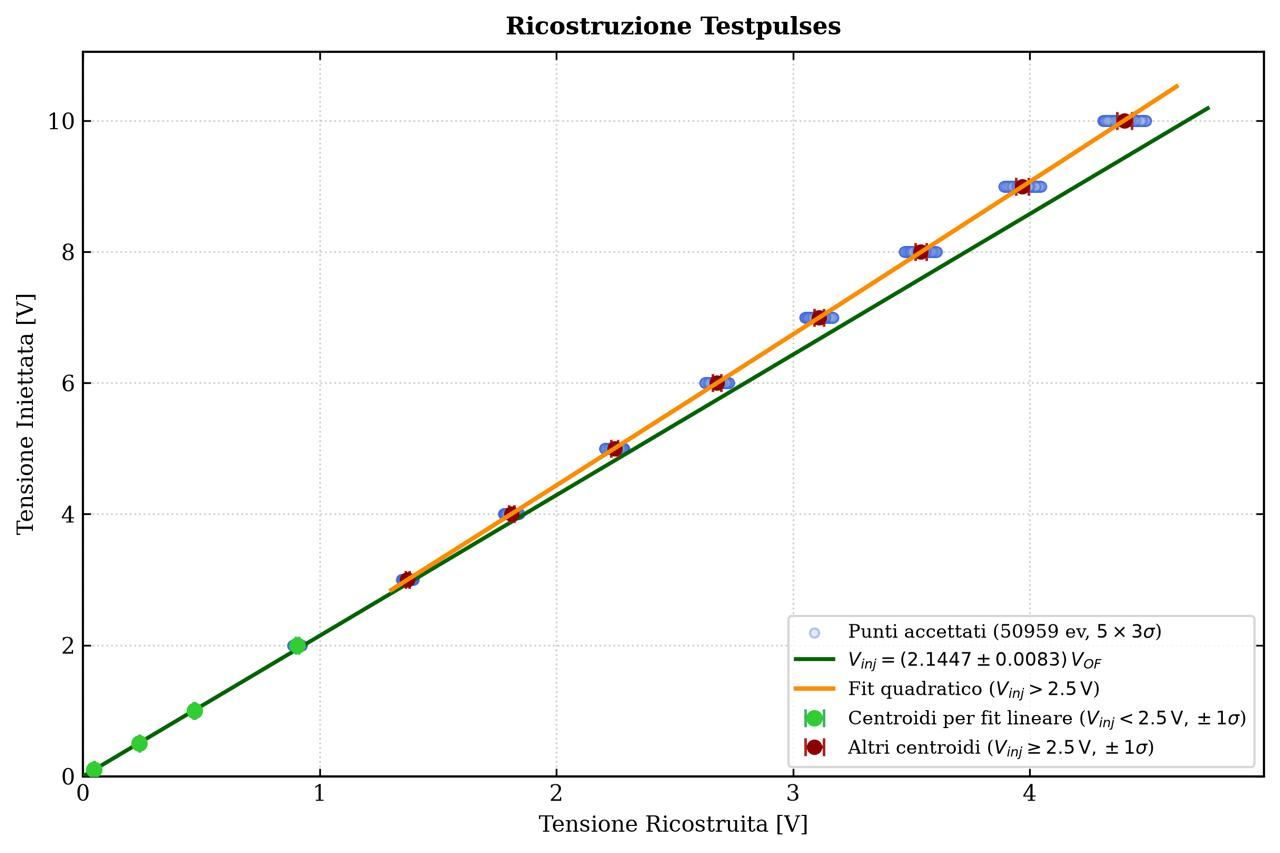
\includegraphics[width=0.75\textwidth]{figures/Ricostruzione_Testpulses.jpeg}
    \caption{Confronto tra le ampiezze stimate con l'Optimum Filter standard e quelle corrette tramite la procedura di ricostruzione su impulsi troncati di \texttt{cait}. La linea verde rappresenta l'estrapolazione lineare dei punti non saturi a bassa energia, mentre la curva arancione, eseguita tramite fit con un polinomio di secondo grado, illustra la funzione che verrà utilizzata per linearizzare la risposta del sistema.}
    \label{fig:Ricostruzione_Testpulses}
\end{figure}

Per correggere questa non-linearità residua, conoscendo l'ampiezza ricostruita da \texttt{cait} e volendo ottenere quella reale è sufficiente spostarsi orizzontalmente dal punto sul polinomio di secondo grado fino ad intercettare la retta. Il valore sull'asse delle ascisse ottenuto dall'intersezione rappresenta la vera ampiezza dell'evento nel caso il rivelatore fosse lineare in tutta la sua curva di transizione.

\section{Estrazione dei Picchi e Curva di Calibrazione}
\label{sec:estrazione_picchi}

Completata la catena di linearizzazione strumentale, si procede all'identificazione dei picchi di calibrazione prodotti dalla sorgente di $^{57}\text{Co}$. A tale scopo sono stati selezionati tutti gli eventi saturi registrati sul rivelatore TUM93A e ne è stata ricostruita l'ampiezza corretta secondo la procedura discussa.

L'istogramma delle ampiezze ricostruite è riportato in Figura~\ref{fig:Ricostruzione_Cobalto}. La corretta identificazione delle strutture spettrali viene effettuata mediante il confronto diretto con lo spettro energetico teorico atteso per un cristallo di tungstato di calcio ($\text{CaWO}_4$) esposto a radiazione da Cobalto-57 (Figura~\ref{fig:picchi_teorici}).

\begin{figure}[htbp]
\centering
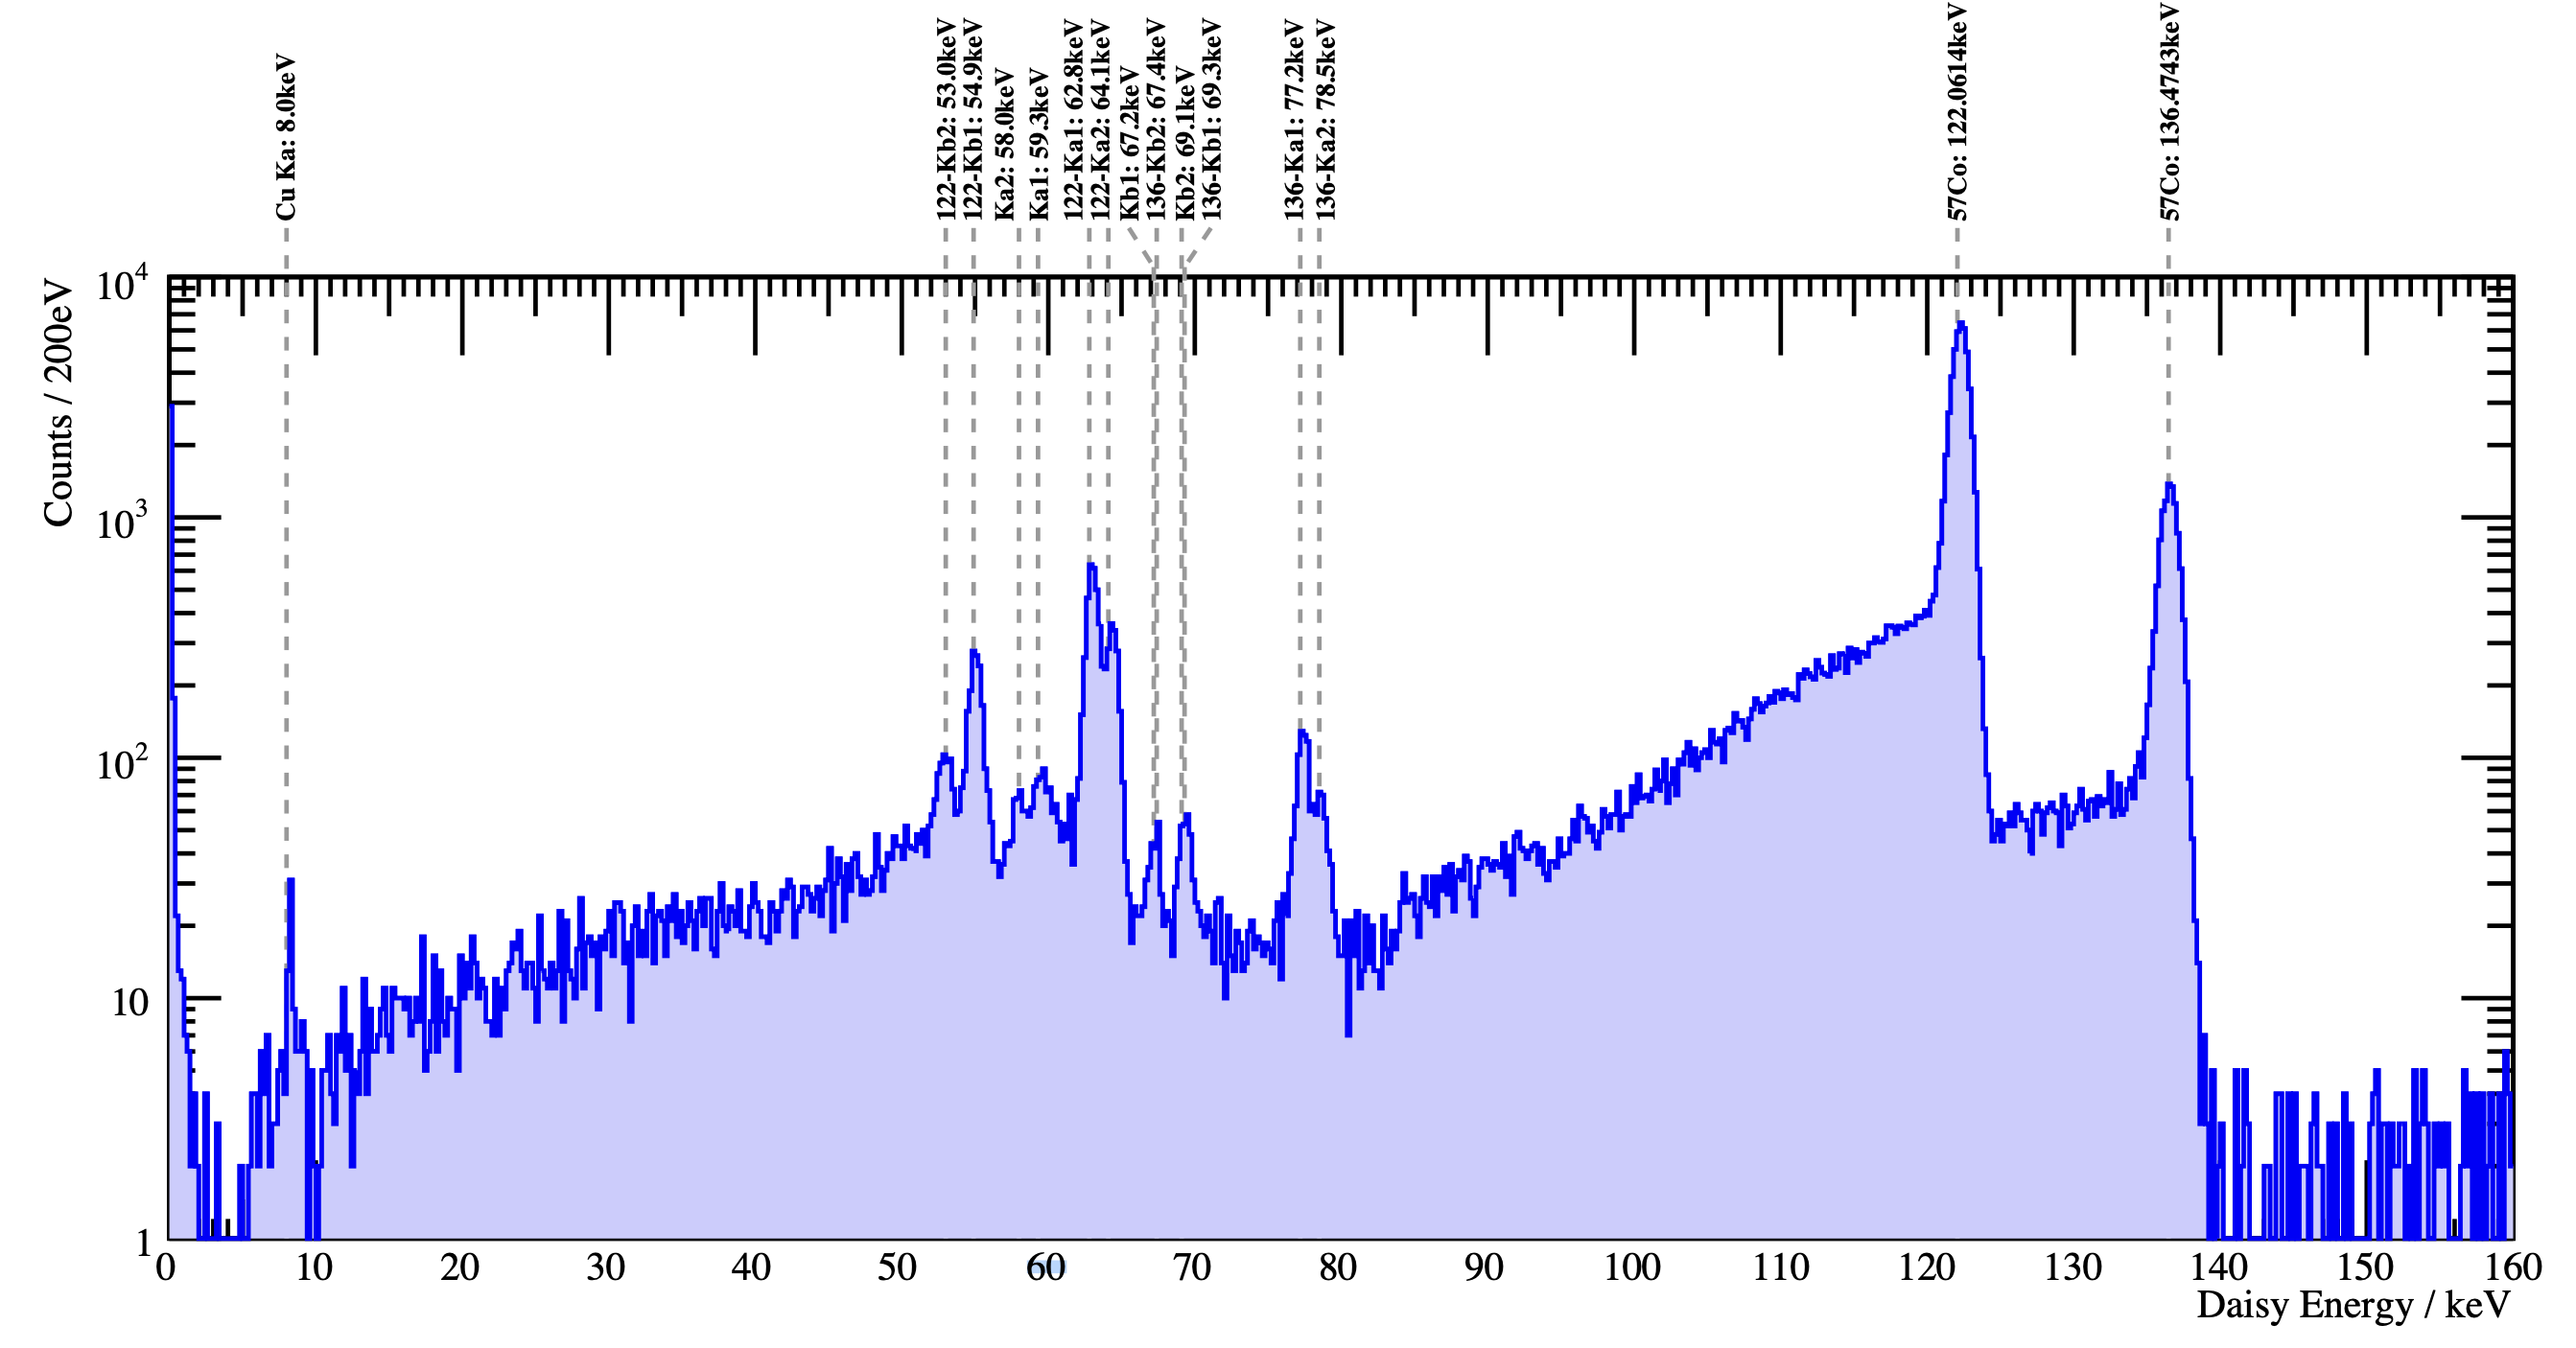
\includegraphics[width=0.8\textwidth]{figures/picchi_teorici.png}
\caption{Spettro energetico teorico atteso nel cristallo per esposizione a una sorgente esterna di $^{57}\text{Co}$. Si distinguono le righe primarie a $122.06\,\text{keV}$ e $136.47\,\text{keV}$, affiancate dal complesso spettro di fluorescenza e dai picchi di fuga del tungsteno compresi nell'intervallo tra $50\,\text{keV}$ e $80\,\text{keV}$.}
\label{fig:picchi_teorici}
\end{figure}

\begin{figure}[htbp]
\centering
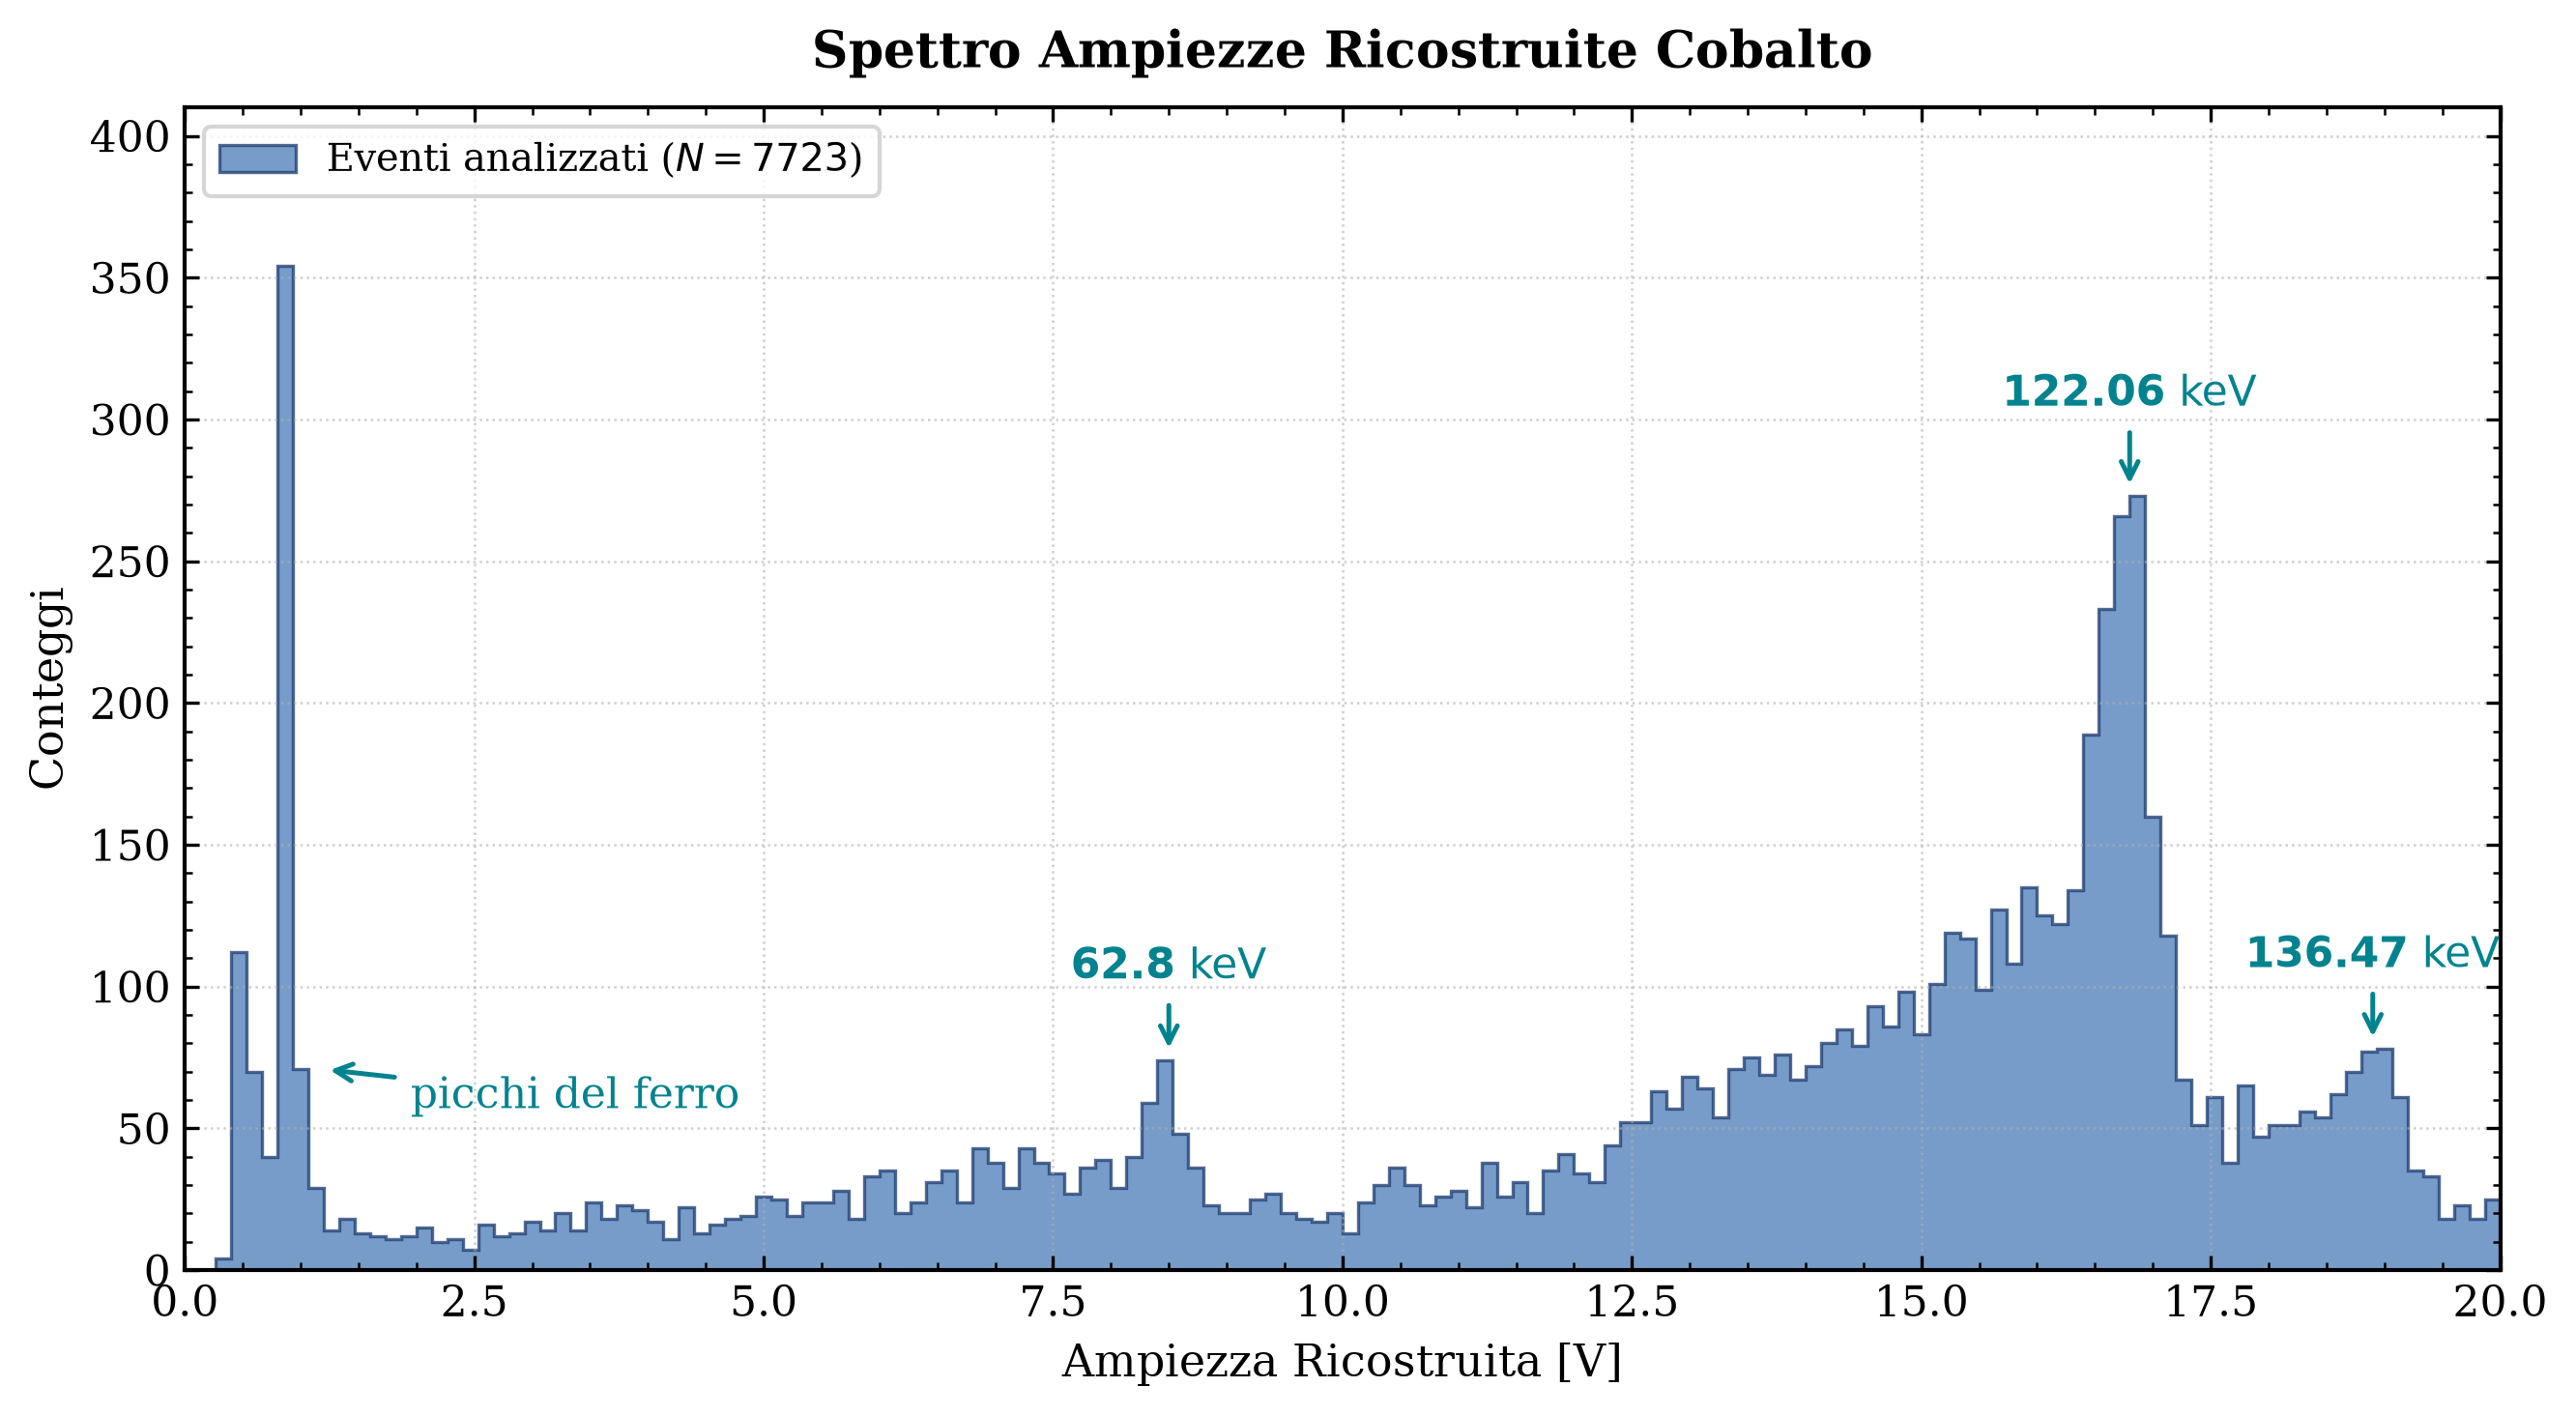
\includegraphics[width=0.8\textwidth]{figures/Spettro_ampiezze_ricostruite.png}
\caption{Spettro sperimentale delle ampiezze ricostruite e corrette per la non-linearità. Si riconoscono chiaramente le due righe principali del Cobalto a circa $19.0\,\text{V}$ e $21.7\,\text{V}$, insieme al picco a circa $9.2\,\text{V}$. Nella regione sub-volt si individua la popolazione corrispondente ai raggi X a circa $6\,\text{keV}$ emessi dal $^{55}\text{Fe}$, contestualmente presente nel criostato.}
\label{fig:Ricostruzione_Cobalto}
\end{figure}

Dal confronto tra lo spettro teorico e la distribuzione sperimentale emergono con chiarezza tre picchi ad alta energia:
\begin{enumerate}
    \item Il doppietto terminale ad alta ampiezza, collocato a circa $19.0\,\text{V}$ e $21.7\,\text{V}$, corrisponde univocamente alle transizioni $\gamma$ principali del $^{57}\text{Co}$ a $122.06\,\text{keV}$ e $136.47\,\text{keV}$;
    \item Nella regione intermedia (tra $8\,\text{V}$ e $11\,\text{V}$), dominata dalle transizioni di fluorescenza del tungsteno, emerge una riga prominente centrata a circa $9.19\,\text{V}$, corrispondente al picco di fuga primario $122 - K_{\alpha_1}$ a $62.8\,\text{keV}$. Gli altri picchi risultano sommersi dal fondo e non è possibile compararli allo spettro atteso;
    \item A bassissime tensioni ($< 1\,\text{V}$) si colloca infine l'emissione del $^{55}\text{Fe}$ ($5.89\,\text{keV}$ e $6.49\,\text{keV}$).
\end{enumerate}

\subsection{Fisica delle sorgenti di calibrazione ($^{57}\text{Co}$ e $^{55}\text{Fe}$)}

Per la calibrazione in energia del rivelatore sono state impiegate due sorgenti radioattive a cattura elettronica: $^{57}\text{Co}$ e $^{55}\text{Fe}$.

\subsubsection*{Emissione del $^{57}\text{Co}$ e interazione nel rivelatore}
Il $^{57}\text{Co}$ ($T_{1/2} \approx 271.7\text{ d}$) decade per cattura elettronica verso stati eccitati del nucleo figlio $^{57}\text{Fe}$, popolando principalmente il secondo livello a $136.47\text{ keV}$. La diseccitazione nucleare avviene attraverso due processi principali:
\begin{itemize}
    \item una transizione diretta allo stato fondamentale con emissione di un fotone $\gamma$ da $136.47\text{ keV}$ (branching ratio del $10.7\%$);
    \item una cascata a due fotoni in cui il nucleo transita prima al livello a $14.41\text{ keV}$ emettendo un fotone $\gamma$ da $122.06\text{ keV}$ ($85.6\%$), seguito dal rilascio del quanto da $14.41\text{ keV}$ verso lo stato fondamentale.
\end{itemize}

I fotoni incidenti a $122\text{ keV}$ e $136\text{ keV}$ interagiscono nel cristallo rivelatore prevalentemente per effetto fotoelettrico sugli elettroni del guscio K del tungsteno ($Z = 74$, $B_K \approx 69.52\text{ keV}$). L'elettrone fotoelettrico espulso porta con sé un'energia cinetica $T_e = E_\gamma - B_K$, interamente rilasciata nel volume.

La lacuna atomica nel guscio K viene colmata tramite riarrangiamento elettronico con conseguente emissione di raggi X di fluorescenza caratteristici del tungsteno:
\begin{itemize}
    \item $K_{\alpha_1}$ ($L_{\text{III}} \to K$): $59.32\text{ keV}$
    \item $K_{\alpha_2}$ ($L_{\text{II}} \to K$): $57.98\text{ keV}$
    \item $K_{\beta_1}$ ($M_{\text{III}} \to K$): $67.24\text{ keV}$
    \item $K_{\beta_2}$ ($N_{\text{III}} \to K$): $69.10\text{ keV}$
\end{itemize}
Nel caso in cui tale fotone X sfugga dal cristallo senza subire ulteriori interazioni, l'energia totale depositata nell'evento è pari alla differenza tra l'energia del $\gamma$ incidente e l'energia del quanto fuggito ($E_{\text{dep}} = E_\gamma - E_X$). Come si osserva nello spettro di Figura~\ref{fig:picchi_teorici}, sottraendo i valori dei raggi X del tungsteno alla riga da $122.06\text{ keV}$ si originano i doppietti di fuga:
\begin{itemize}
    \item $122 - K_{\alpha_1} \approx 62.8\text{ keV}$ e $122 - K_{\alpha_2} \approx 64.1\text{ keV}$;
    \item $122 - K_{\beta_1} \approx 54.9\text{ keV}$ e $122 - K_{\beta_2} \approx 53.0\text{ keV}$.
\end{itemize}
Analogamente, dalla riga a $136.47\text{ keV}$ derivano i picchi di fuga $136 - K_\alpha$ (a circa $77.2$ e $78.5\text{ keV}$) e $136 - K_\beta$ (a $67.4$ e $69.1\text{ keV}$). Nella medesima regione spettrale emergono inoltre i picchi di fluorescenza diretta del tungsteno ($K_\alpha$ a $58.0-59.3\text{ keV}$ e $K_\beta$ a $67.2\text{ keV}$), dovuti a eventi in cui i raggi X generati all'interno o nelle vicinanze del cristallo vengono interamente assorbiti.

\subsubsection*{Emissione del $^{55}\text{Fe}$}
Il $^{55}\text{Fe}$ ($T_{1/2} \approx 2.74\text{ anni}$) decade anch'esso per cattura elettronica, transmutando in un nucleo di $^{55}\text{Mn}$. Il decadimento popola direttamente lo stato fondamentale del $^{55}\text{Mn}$: di conseguenza, non vi è alcuna emissione di fotoni $\gamma$ di origine nucleare.

Il segnale rilevato è invece interamente dovuto alla diseccitazione elettronica dell'atomo figlio: la cattura di un elettrone orbitale crea prevalentemente una vacanza nel guscio K del manganese ($B_K = 6.54\text{ keV}$). Il riempimento radiativo di questa lacuna genera due caratteristiche righe X:
\begin{itemize}
    \item la riga $K_\alpha$ a $5.89\text{ keV}$, corrispondente alla transizione di un elettrone dal guscio L al guscio K ($2p \to 1s$);
    \item la riga $K_\beta$ a $6.49\text{ keV}$, associata alla transizione dal guscio M al guscio K ($3p \to 1s$).
\end{itemize}
Queste due righe forniscono un preciso punto di ancoraggio per la calibrazione nella regione delle basse energie.

\subsection{Fit dei picchi del Cobalto e del Ferro}
\label{subsec:fit_picchi_cobalto}

La determinazione precisa delle ampiezze corrispondenti alle righe del $^{57}\text{Co}$ richiede un modello spettrale che tenga conto della complessa risposta sperimentale del calorimetro. 

\subsubsection*{Doppietto ad alta energia ($122.06\text{ keV}$ e $136.47\text{ keV}$)}
L'ispezione dei due foto-picchi ad alta ampiezza (Figura~\ref{fig:Ricostruzione_Cobalto}) mostra chiaramente che una semplice funzione gaussiana risulta inadeguata: a sinistra di ciascun picco, il livello dei conteggi si assesta a una quota sensibilmente superiore rispetto alla linea di base alla sua destra. Tale asimmetria è dovuta allo scattering Compton negli schermi: parte dei fotoni $\gamma$ primari subisce diffusione Compton sugli elettroni dei materiali interposti (schermature di piombo, pareti in rame e schermi termici del criostato) prima di raggiungere il cristallo, arrivando con energia degradata e originando una coda continua di eventi al di sotto del picco di assorbimento totale;

Per modellizzare accuratamente questa forma di riga è stata impiegata una funzione 
analitica composita basata sulla parametrizzazione di tipo \textit{Crystal Ball} \cite{Skwarnicki:1986}, estesa con un termine a gradino derivato dall'effetto Compton. Introducendo per ciascun picco $k \in \{1, 2\}$ la variabile ridotta centrata e normalizzata:
\begin{equation}
    u_k = \frac{x - \mu_k}{\sigma_k},
\end{equation}
dove $\mu_k$ rappresenta la posizione del picco e $\sigma_k$ la dispersione gaussiana associata alla risoluzione strumentale, il profilo del picco $P_k(u_k)$ è definito a tratti:
\begin{equation}
    P_k(u_k) = 
    \begin{cases} 
        A_k \exp\left(-\frac{1}{2} u_k^2\right), & \text{per } u_k \ge -\tau_k \\[6pt]
        A_k \exp\left(\frac{1}{2} \tau_k^2 + \tau_k u_k\right), & \text{per } u_k < -\tau_k
    \end{cases}
\end{equation}
dove $\tau_k > 0$ è il parametro adimensionale che definisce la soglia di transizione (in unità di deviazioni standard a sinistra del centro) in cui la campana gaussiana si raccorda, con continuità di funzione e derivata prima, a una coda di decadimento esponenziale.

A questa componente di picco viene sommato il contributo a gradino (\textit{step function}), che descrive l'innalzamento della linea di base a sinistra dovuto al continuo Compton. Matematicamente, tale gradino è espresso dalla convoluzione di una funzione a gradino di Heaviside con la funzione di risoluzione gaussiana del calorimetro, traducendosi nella funzione degli errori complementare ($\mathrm{erfc}$):
\begin{equation}
    S_k(u_k) = \frac{1}{2} A_{\text{step}, k} \, \mathrm{erfc}\left(\frac{u_k}{\sqrt{2}}\right).
\end{equation}

Il modello complessivo include inoltre un fondo residuo comune descritto da una costante ($B(x) = p_0$), per un totale di 11 parametri liberi (5 per ciascun picco e 1 per il fondo). L'espressione finale del modello di fit è quindi:
\begin{equation}
    F(x) = B(x) + \sum_{k=1}^{2} \Big[ P_k(u_k(x)) + S_k(u_k(x)) \Big].
\end{equation}

\begin{figure}[htbp]
    \centering
    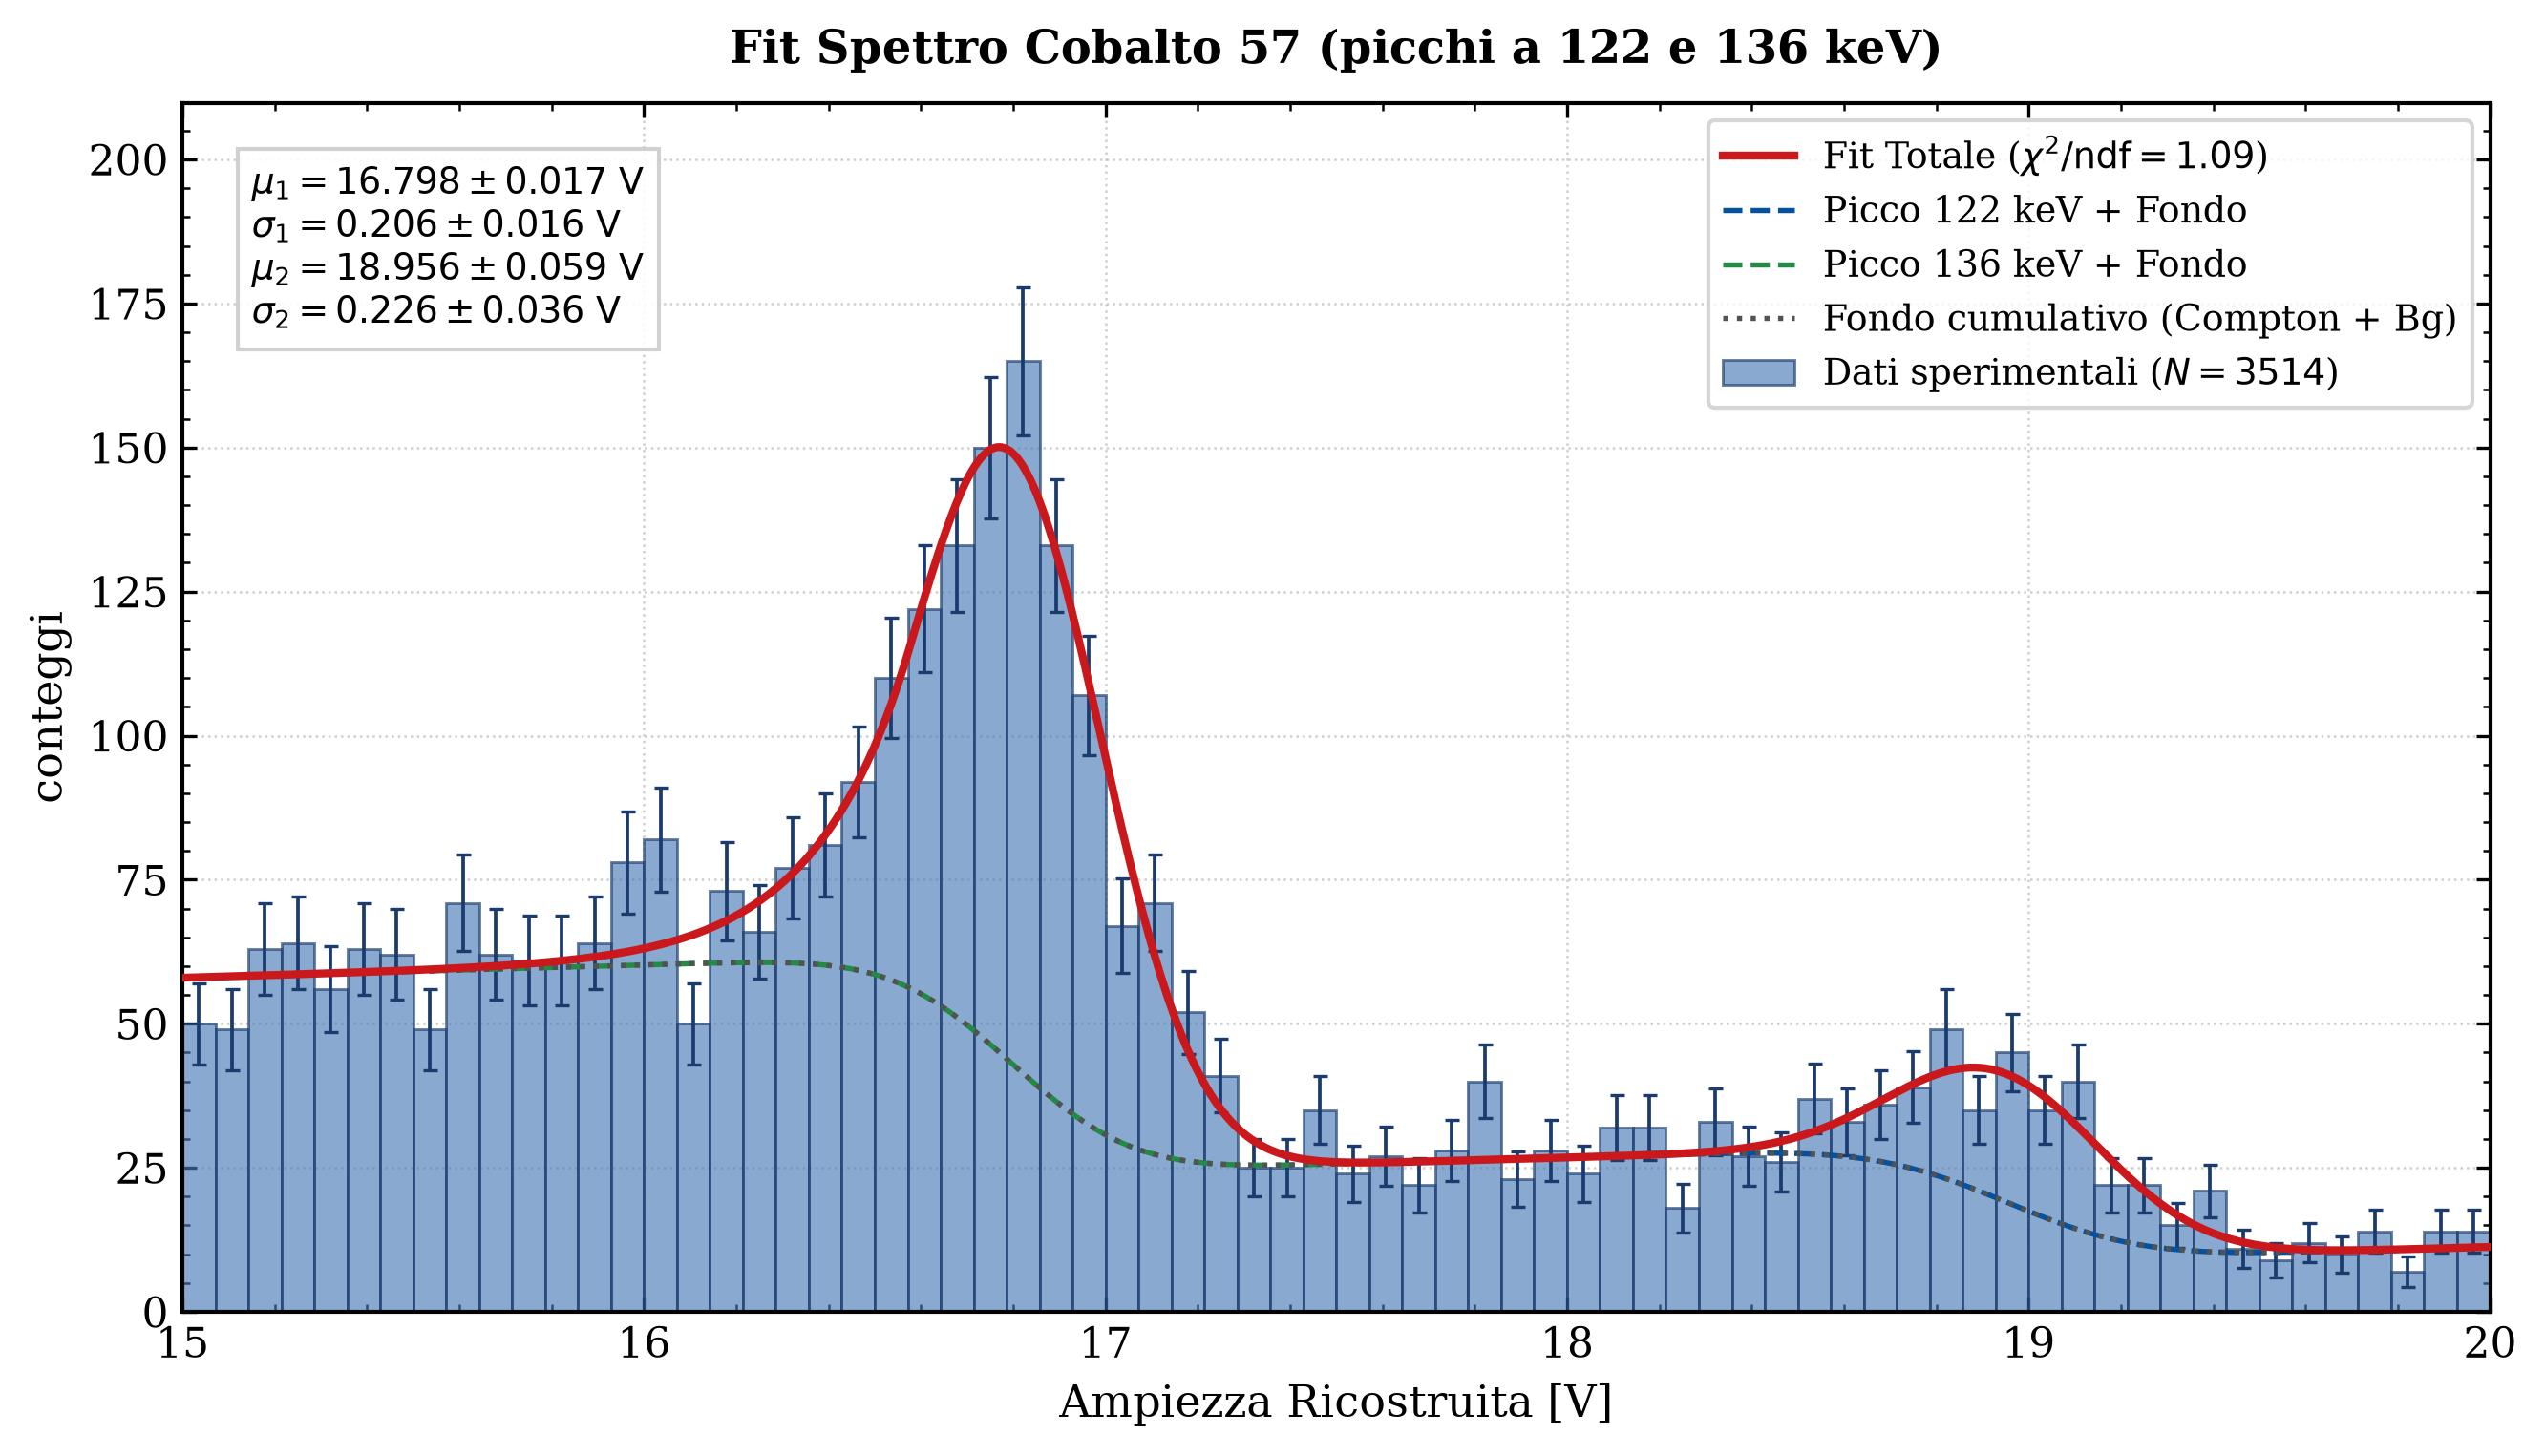
\includegraphics[width=0.85\textwidth]{figures/fit_57Co_122_136keV.jpeg}
    \caption{Fit congiunto delle righe $\gamma$ del $^{57}\text{Co}$ a $122.06\,\text{keV}$ e $136.47\,\text{keV}$ mediante modello Crystal Ball con coda esponenziale a sinistra, gradino $\mathrm{erfc}$ e fondo lineare comune.}
    \label{fig:Ricostruzione_Cobalto}
\end{figure}

Il fit è stato eseguito minimizzando la statistica del $\chi^2$ su un istogramma suddiviso in 70 bin:
\begin{equation}
    \chi^2 = \sum_{i=1}^{70} \frac{\left( N_i^{\text{oss}} - N_i^{\text{att}}(F) \right)^2}{\sigma_i^2},
\end{equation}
dove $N_i^{\text{oss}}$ rappresenta il conteggio osservato nel bin $i$-esimo, $N_i^{\text{att}}$ il valore predetto dall'integrazione del modello e $\sigma_i = \sqrt{N_i^{\text{oss}}}$ l'incertezza poissoniana associata. Con $70 - 11 = 59$ gradi di libertà, il fit converge con un $\chi^2_{\text{red}} \approx 1$, a conferma dell'eccellente capacità del modello di riprodurre la fisica del segnale. I parametri fondamentali estratti dalla minimizzazione sono:
\begin{itemize}
    \item Picco $122.06\text{ keV}$: $\mu_1 = 16.80 \pm 0.02\,\text{V}$, \quad $\sigma_1 = 0.21 \pm 0.02\,\text{V}$;
    \item Picco $136.47\text{ keV}$: $\mu_2 = 18.96 \pm 0.03\,\text{V}$, \quad $\sigma_2 = 0.23 \pm 0.02\,\text{V}$.
\end{itemize}

\subsubsection*{Picco di fuga del Tungsteno ($62.8\text{ keV}$)}
L'identificazione del picco di fuga $122 - K_{\alpha_1}$ a $62.8\,\text{keV}$ risulta più complessa, in quanto la struttura spettrale emerge su un continuo di eventi di scattering notevolmente più denso rispetto alla regione ad alta ampiezza.

Per incrementare la purezza del campione ed eliminare eventuali interazioni spurie o particelle cariche di fondo, è stata preliminarmente analizzata la distribuzione del \textit{Light Yield} ($LY$), definito dal rapporto tra l'energia rilevata nel canale luminoso e quella depositata nel canale fononico ($LY = E_{\text{luce}} / E_{\text{calore}}$), riportata in Figura~\ref{fig:Light_Yield}. 

\begin{figure}[htbp]
    \centering
    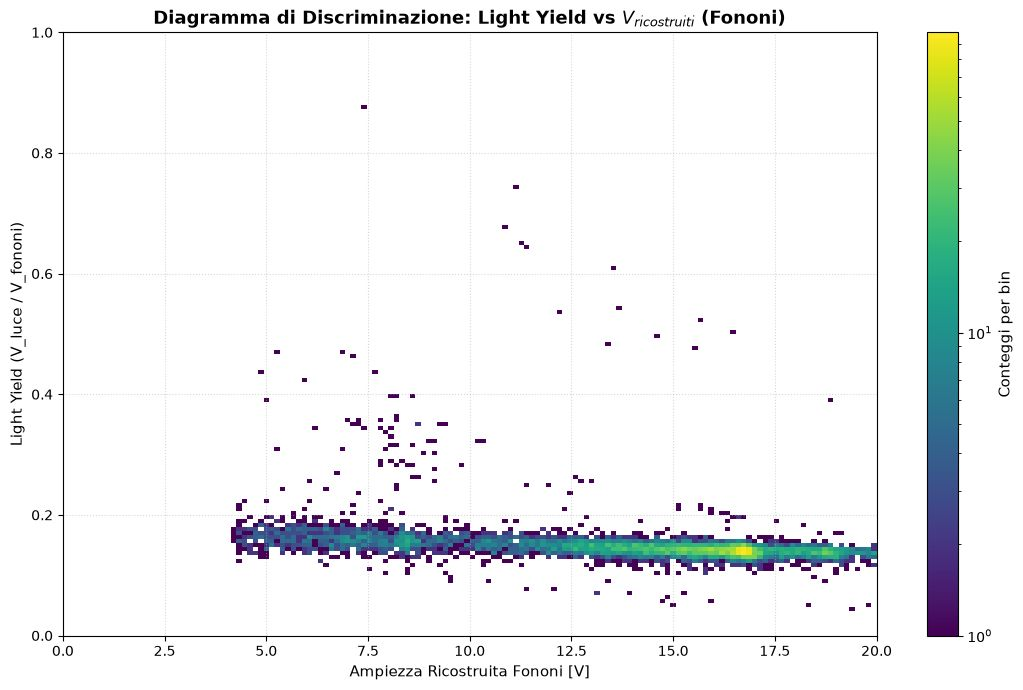
\includegraphics[width=0.8\textwidth]{figures/grafico_LY.jpeg}
    \caption{Distribuzione bidimensionale del Light Yield in funzione della tensione ricostruita. La popolazione principale evidenzia la banda elettronica ($e^-/\gamma$), caratterizzata da un rapporto di scintillazione sostanzialmente uniforme lungo l'intero intervallo energetico.}
    \label{fig:Light_Yield}
\end{figure}

Come illustrato dal grafico, gli eventi associati a rinculi elettronici ($e^-/\gamma$) si concentrano lungo una banda ben definita con $LY \approx 0.2$. Applicando un taglio selettivo a $\pm 3\sigma$ attorno al baricentro di tale banda, sono stati scartati gli eventi con rapporto anomalo.

\begin{figure}[htbp]
    \centering
    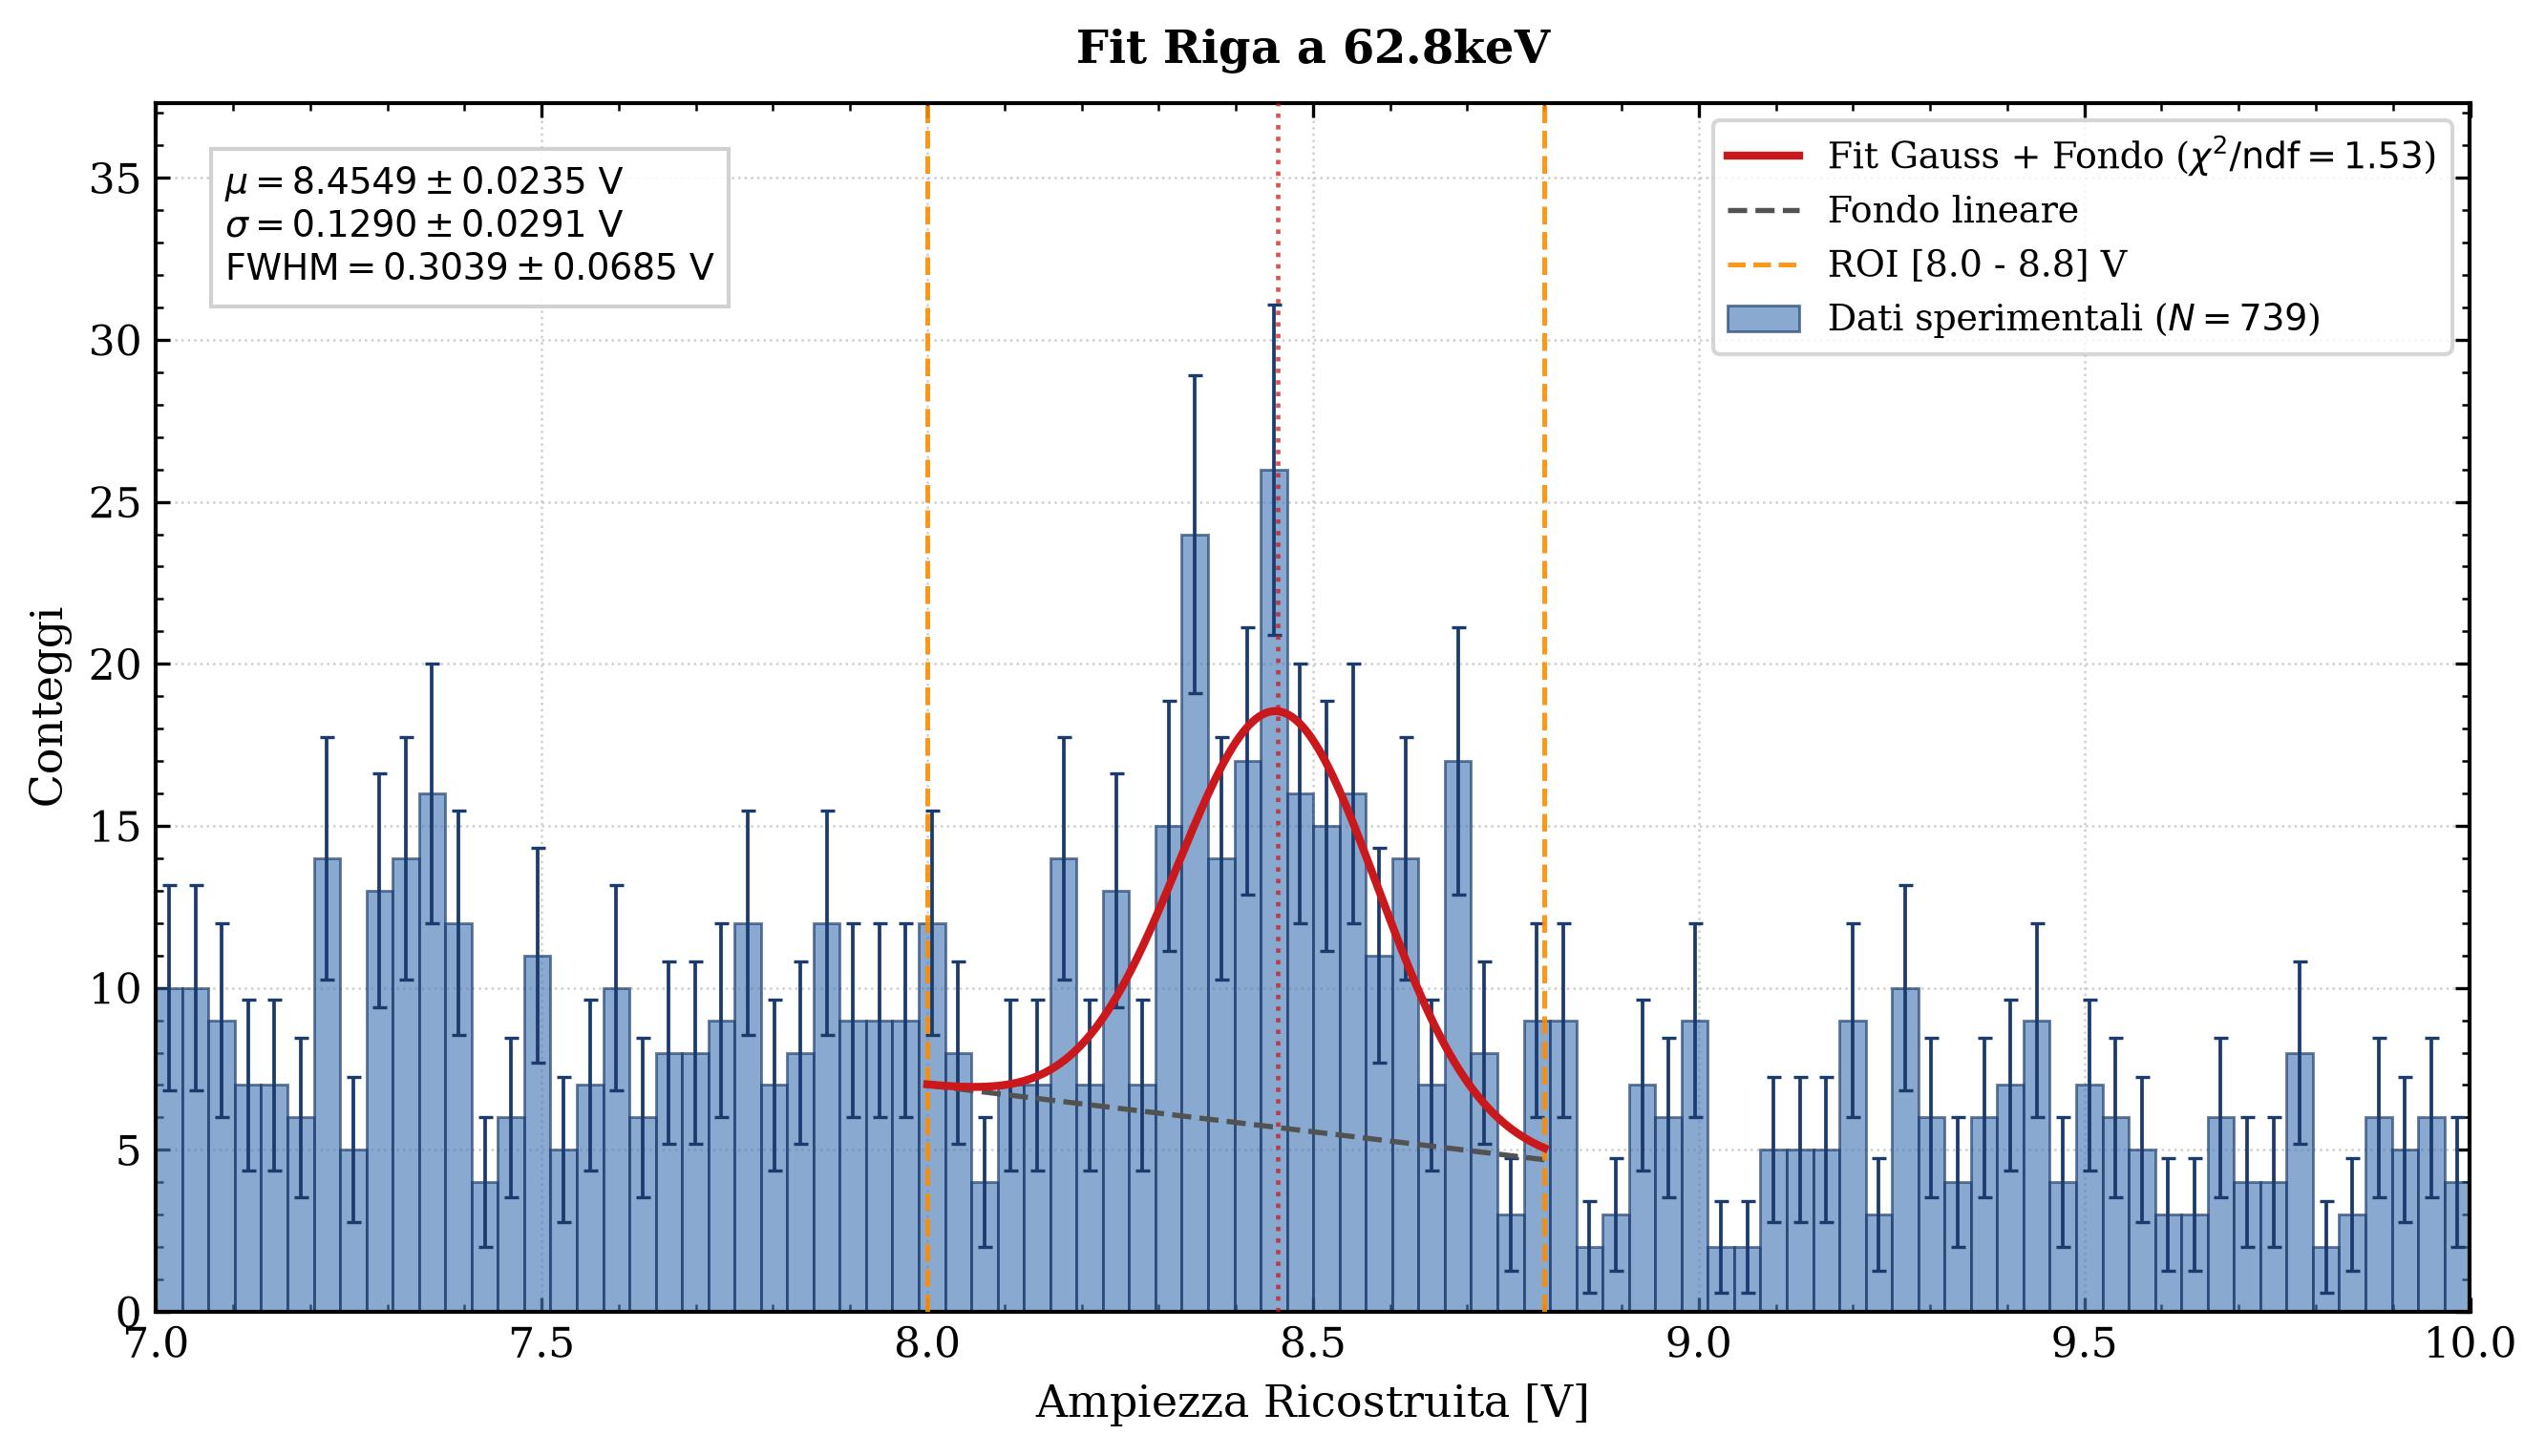
\includegraphics[width=0.8\textwidth]{figures/Fit_riga_centrale.jpeg}
    \caption{Fit del picco di fuga del tungsteno a $62.8\,\text{keV}$ ristretto alla regione di interesse compresa tra $8.0\,\text{V}$ e $8.8\,\text{V}$. Il modello comprende una gaussiana per il picco e un fondo polinomiale di primo grado.}
    \label{fig:Fit_riga_centrale}
\end{figure}

Poiché nella regione compresa tra $50\,\text{keV}$ e $80\,\text{keV}$ coesistono molteplici transizioni minori, l'analisi è stata circoscritta a una ristretta Regione di Interesse (ROI) attorno alla riga da $62.8\,\text{keV}$ (intervallo $8.0 - 8.8\,\text{V}$). In questa finestra locale, l'andamento è stato descritto tramite la combinazione di una singola funzione gaussiana e un fondo lineare:
\begin{equation}
    f_{\text{ROI}}(x) = \frac{A_3}{\sqrt{2\pi}\sigma_3} \exp\left( -\frac{(x - \mu_3)^2}{2\sigma_3^2} \right) + (c_0 + c_1 x).
\end{equation}
La minimizzazione ha condotto a una determinazione statisticamente solida del centroide del picco:
\begin{itemize}
    \item Picco $62.8\text{ keV}$: $\mu_3 = 8.45 \pm 0.03\,\text{V}$, \quad $\sigma_3 = 0.13 \pm 0.02\,\text{V}$.
\end{itemize}

\subsubsection*{Picchi del Ferro ($5.89\text{ keV}$ e $6.49\text{ keV}$)}
\label{subsec:fit_picchi_ferro}
Per il fit dei picchi del Ferro, la procedura è stata analoga a quella descritta per il picco di fuga del tungsteno. La regione di interesse è stata limitata all'intervallo $0.8 - 1.0\,\text{V}$, dove si collocano le due righe principali del $^{55}\text{Fe}$. Il modello di fit comprende due gaussiane sovrapposte per i picchi $K_\alpha$ e $K_\beta$, insieme a un fondo lineare. Viene imposto il vincolo che le sigma dei due picchi siano uguali per due motivi:
\begin{enumerate}
    \item l'allargamento della riga è principalmente determinato dalla risoluzione strumentale del calorimetro, che non dipende dall'energia del fotone incidente, che quindi può essere considerata costante per entrambe le transizioni;
    \item la popolazione di eventi a bassa energia è limitata, impostare un altro parametro libero sul fit della seconda gaussiana rischierebbe di allargarla eccessivamente per minimizzare il chi quadro.
\end{enumerate}
\begin{figure}[htbp]
    \centering
    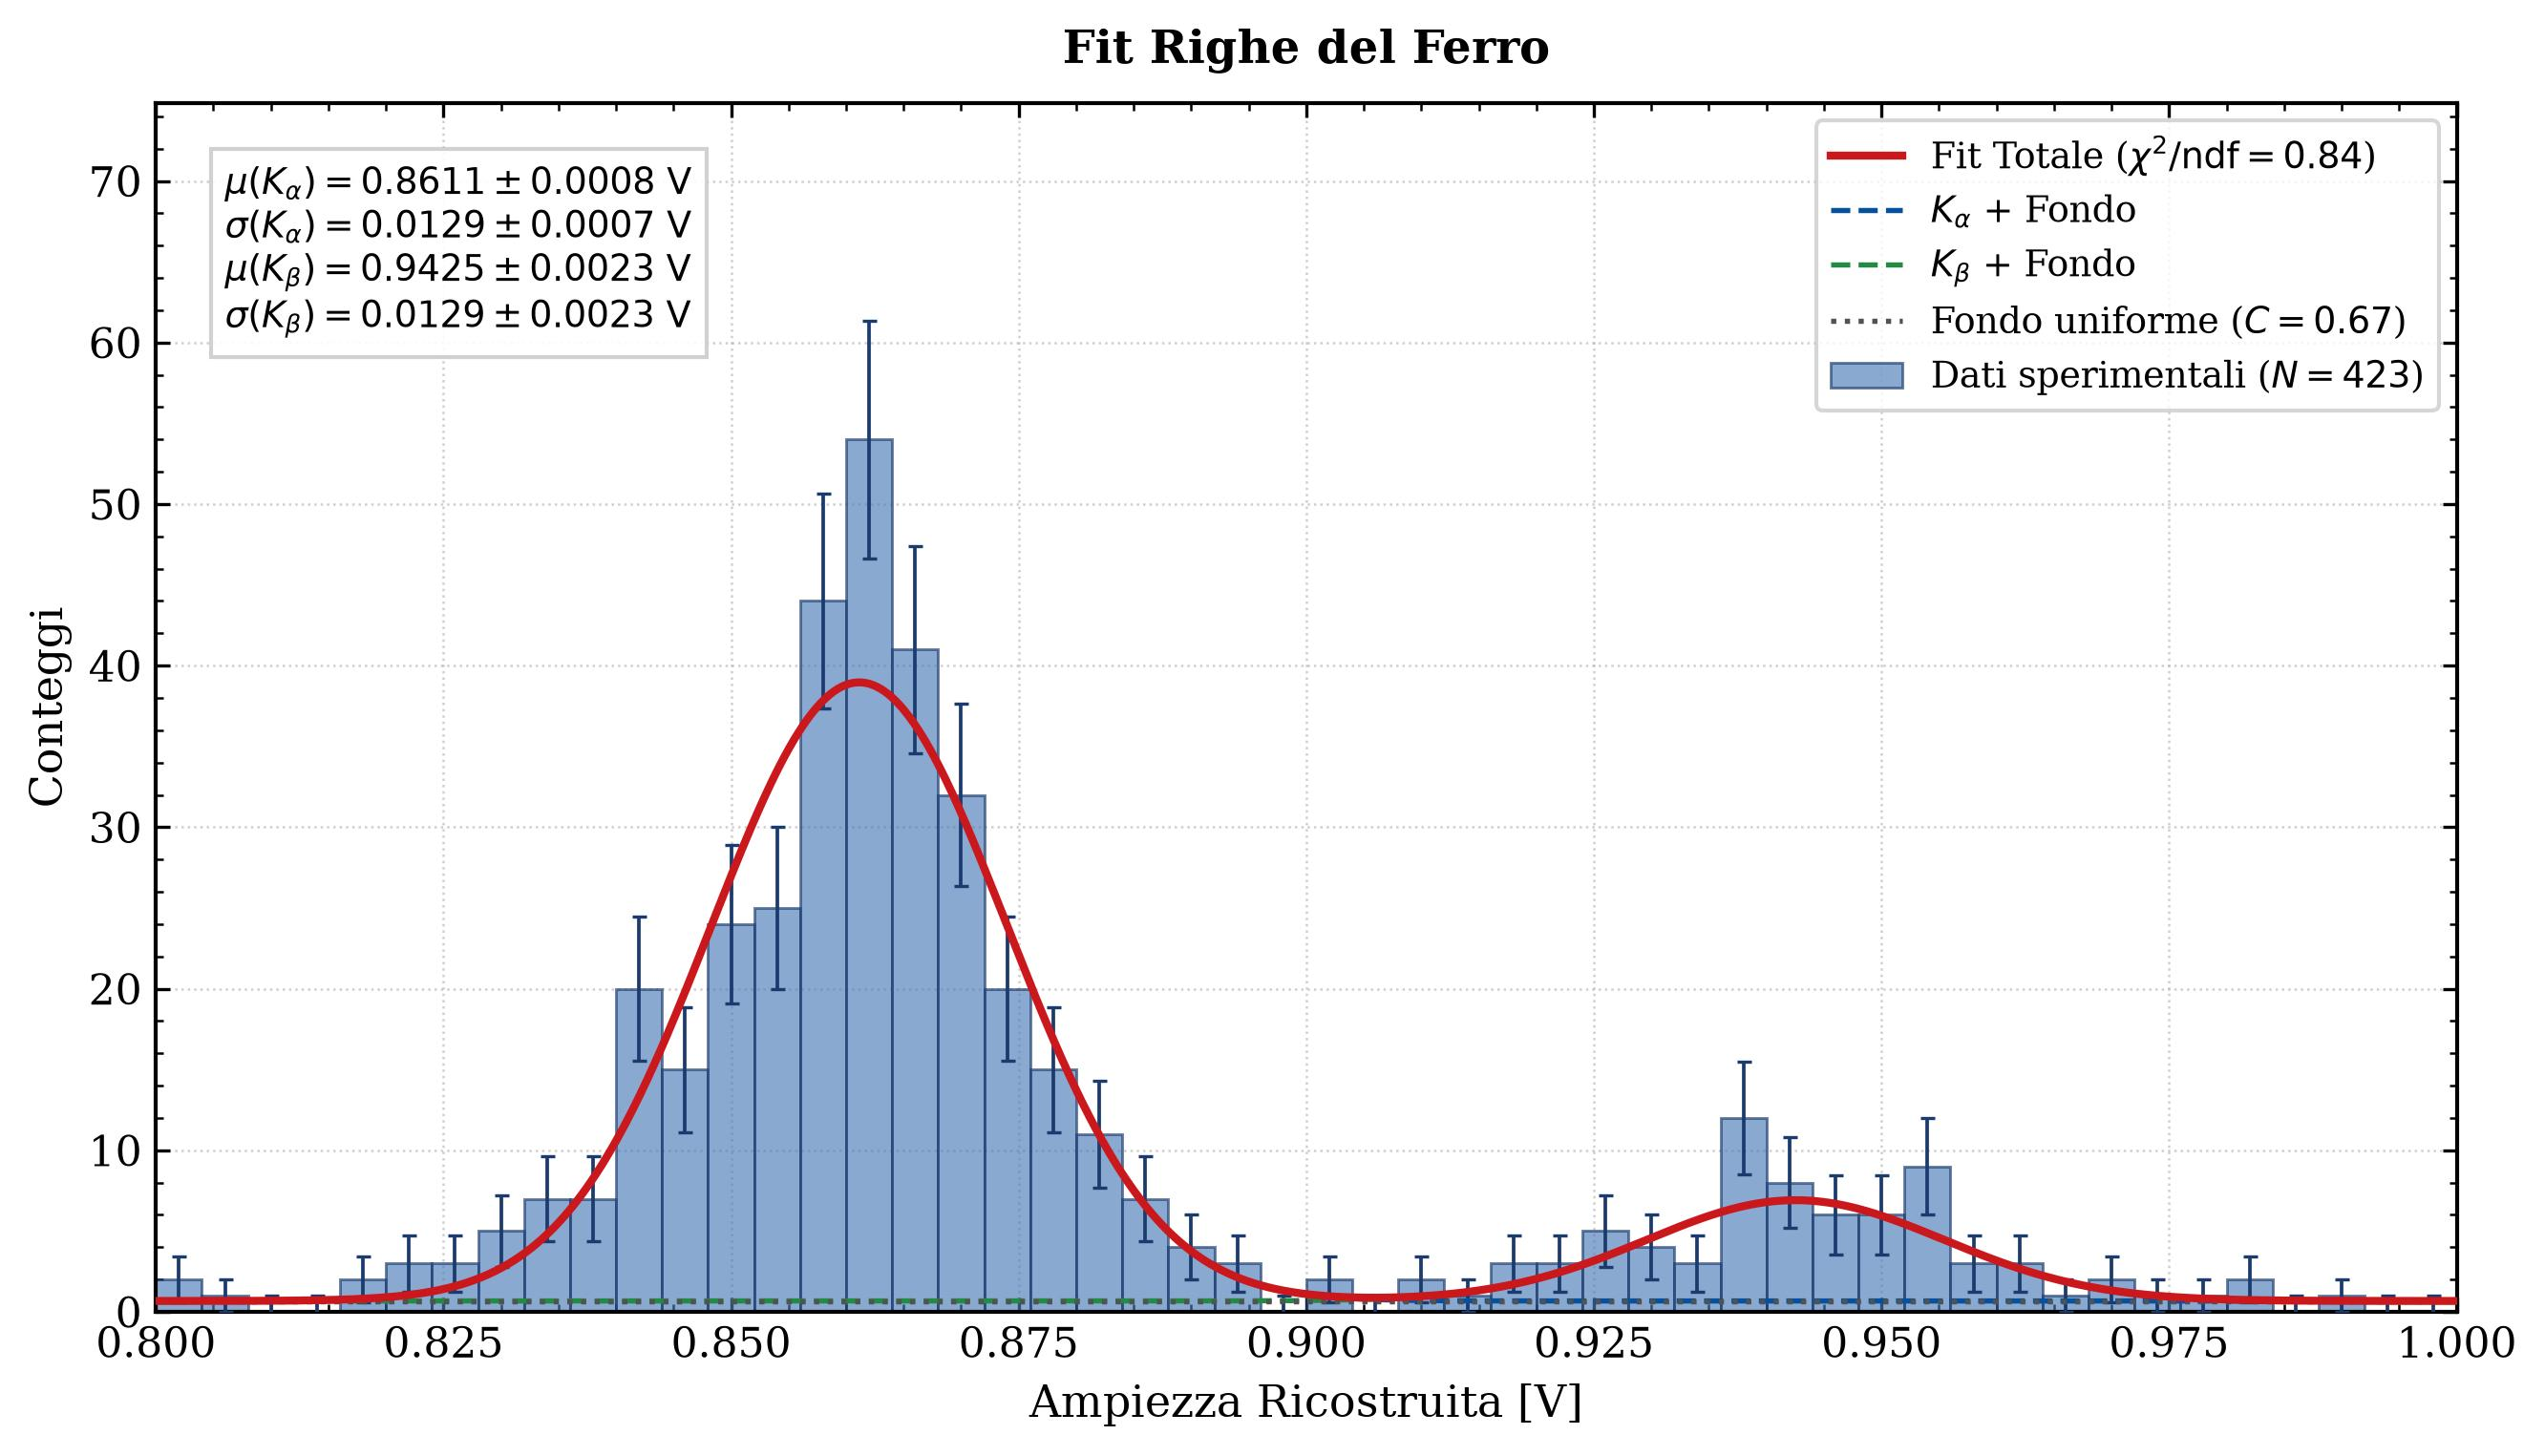
\includegraphics[width=0.8\textwidth]{figures/Fit_righe_Ferro.jpeg}
    \caption{Fit del doppietto del Ferro.}
    \label{fig:Fit_riga_centrale}
\end{figure}
La posizione dei picchi è:
\begin{itemize}
    \item Picco $K_\alpha$ ($5.89\text{ keV}$): $\mu_1 = 0.861 \pm 0.001\,\text{V}$, \quad $\sigma_1 = 0.013 \pm 0.001\,\text{V}$;
    \item Picco $K_\beta$ ($6.49\text{ keV}$): $\mu_2 = 0.943 \pm 0.002\,\text{V}$, \quad $\sigma_2 = 0.013 \pm 0.002\,\text{V}$.
\end{itemize}

\subsection{Linearizzazione delle Ampiezze e Costruzione della Curva di Calibrazione}
\label{subsec:linearizzazione_calibrazione}

Come discusso nel Paragrafo~\ref{subsec:Analisi_Testpulses_ricostruiti}, l'algoritmo di ricostruzione su impulsi troncati presenta una progressiva sottostima sistematica dell'ampiezza al crescere dell'energia depositata. Prima di poter determinare la funzione di risposta energetica del calorimetro, è stato pertanto necessario linearizzare le ampiezze stimate da \texttt{cait} ($V_{\text{rec}}$), proiettandole sulla scala di proporzionalità ideale definita dai testpulse a bassissima energia ($V_{\text{inj}} < 2.5\,\text{V}$).

La procedura geometrica di linearizzazione è illustrata in Figura~\ref{fig:Ricostruzione_picchi_cobalto}:
\begin{figure}[htbp]
    \centering
    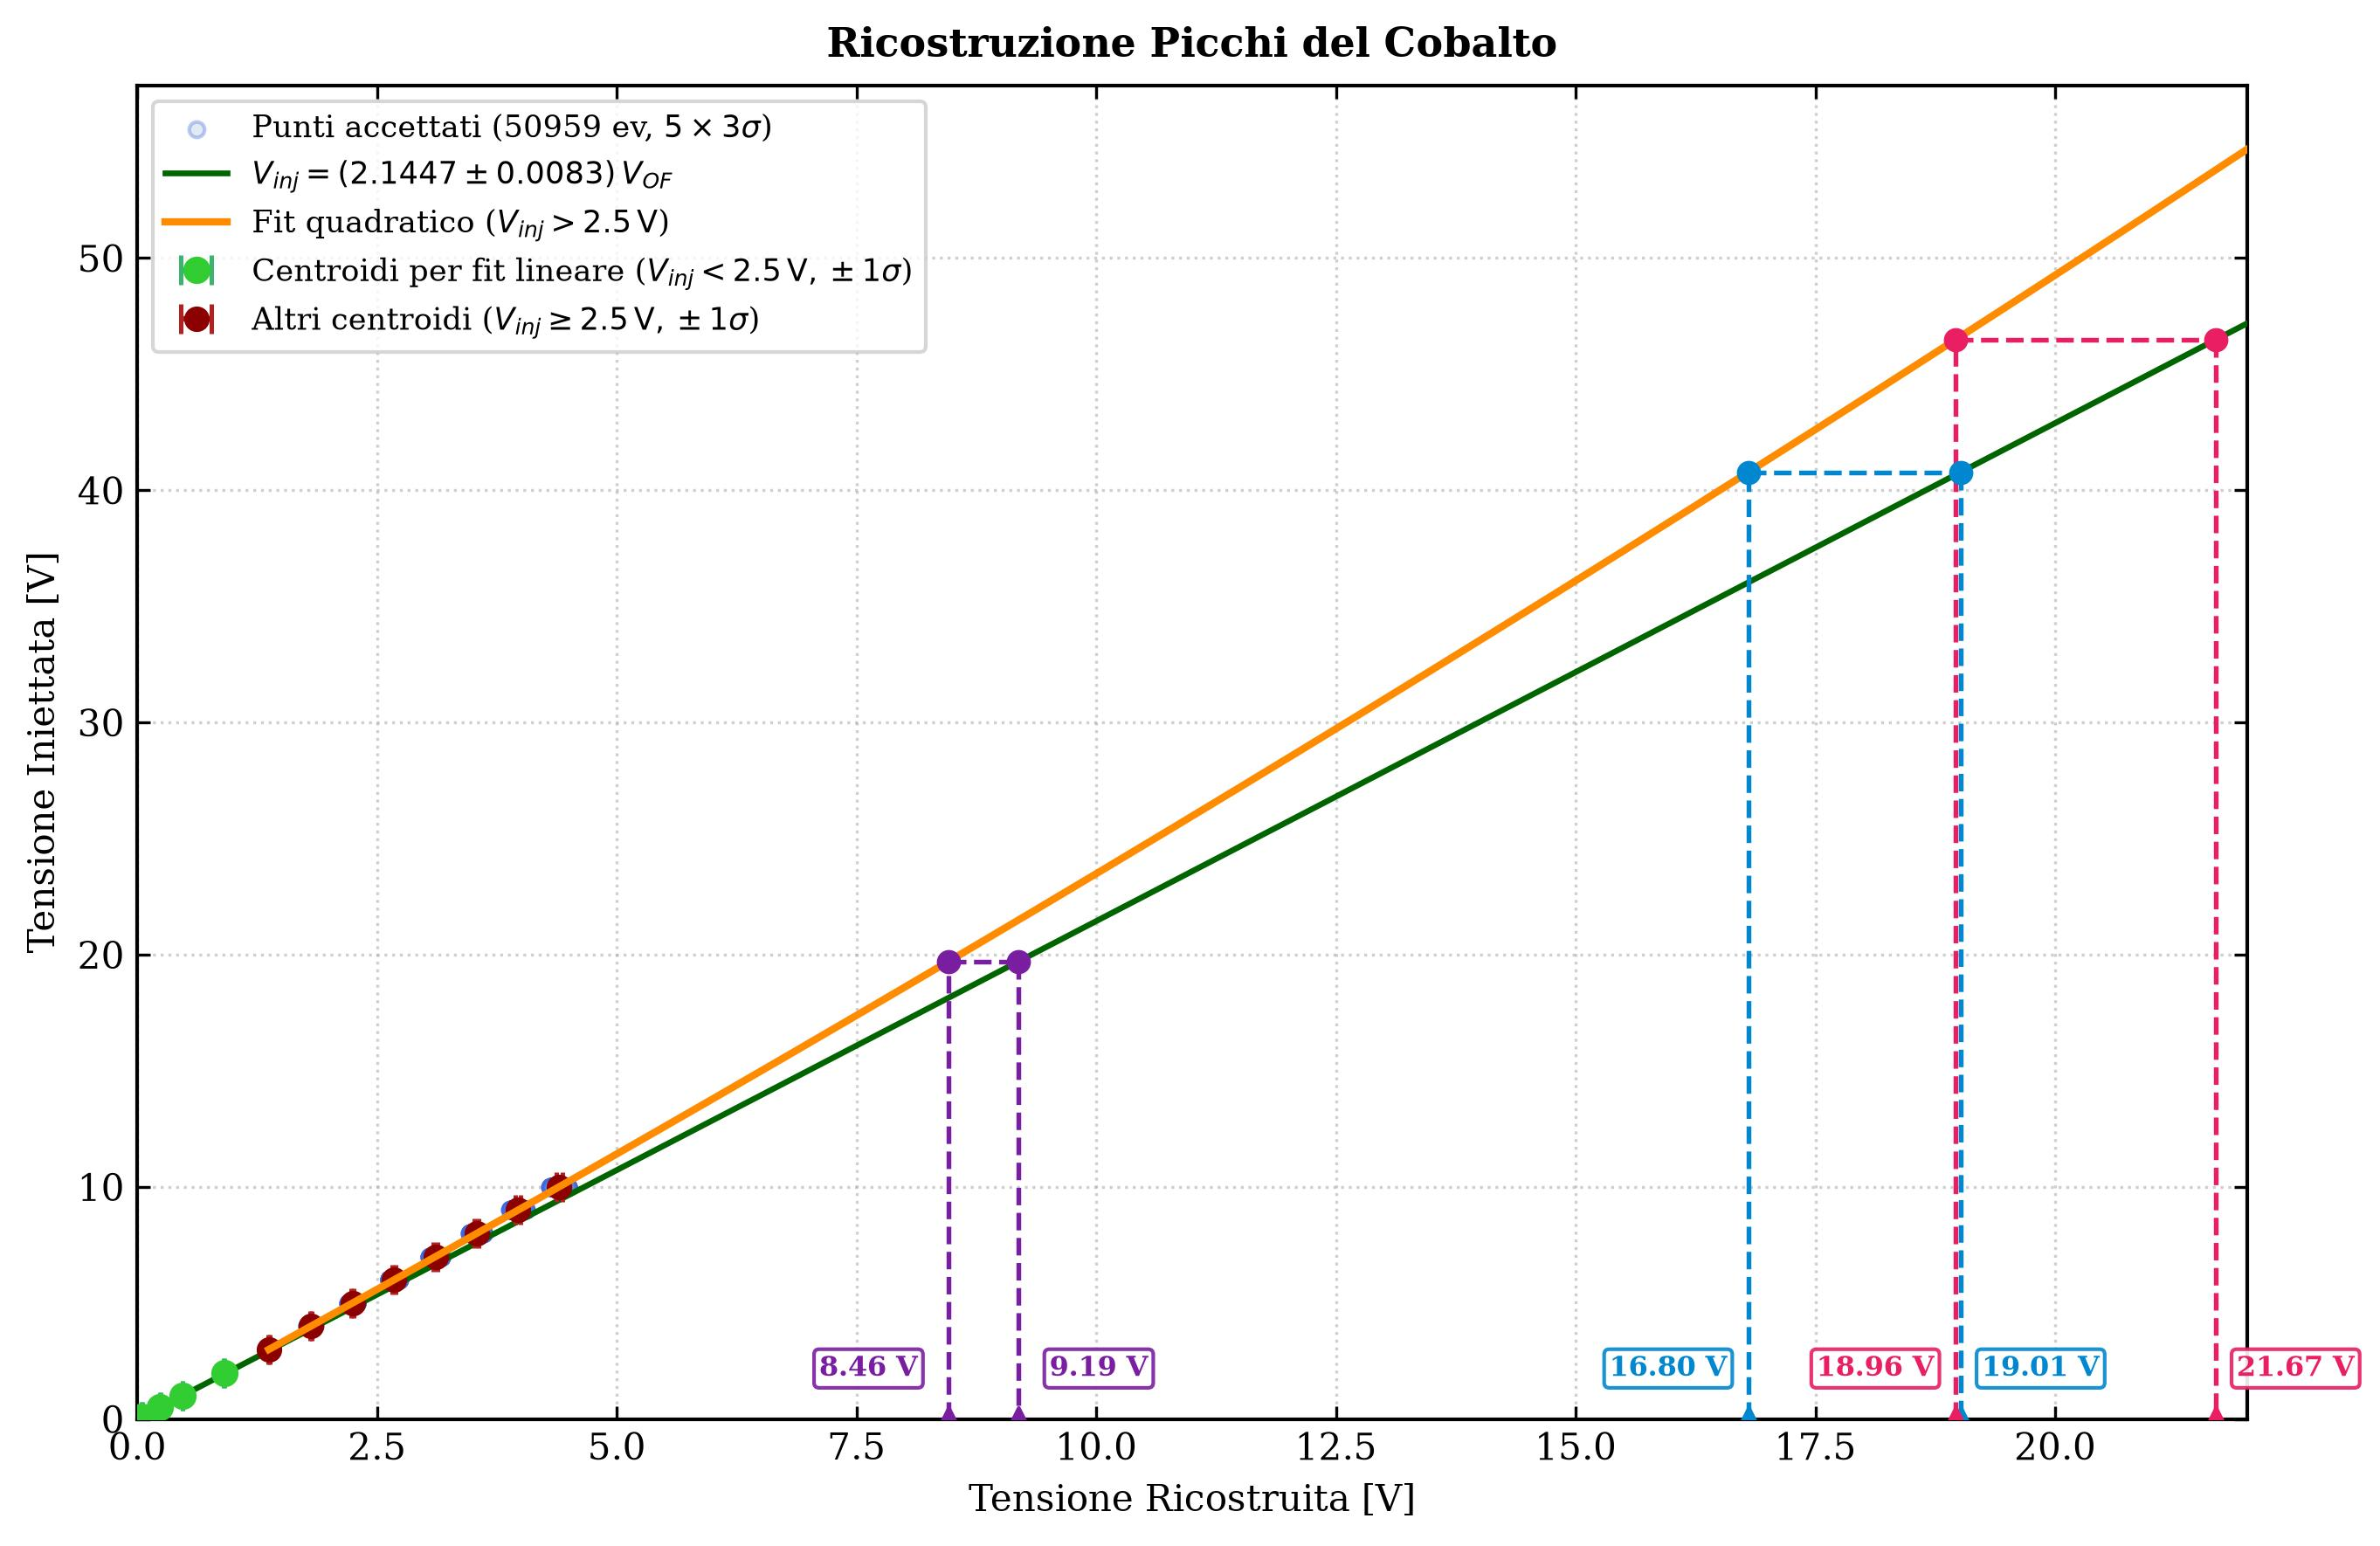
\includegraphics[width=0.88\textwidth]{figures/Ricostruzione_picchi_cobalto.jpeg}
    \caption{Procedura di linearizzazione delle ampiezze stimate per i picchi del $^{57}\text{Co}$. Ciascun valore di tensione ricostruito da \texttt{cait} ($8.46\,\text{V}$, $16.80\,\text{V}$, $18.96\,\text{V}$) viene intercettato sulla curva quadratica dei testpulse (in arancione) e traslato orizzontalmente fino alla retta di risposta lineare ideale a bassa energia (in verde), fornendo le tensioni linearizzate corrette ($9.19\,\text{V}$, $19.01\,\text{V}$, $21.67\,\text{V}$).}
    \label{fig:Ricostruzione_picchi_cobalto}
\end{figure}

Per determinare l'incertezza globale $\sigma_V$ da associare a ciascuna ampiezza linearizzata, sono stati considerati tre contributi indipendenti:
\begin{enumerate}
    \item \textbf{Incertezza statistica del fit spettrale ($\sigma_{\text{stat}}$):} l'incertezza sulla posizione del centroide estratta dal fit dei picchi (la deviazione standard del modello Crystal Ball o della gaussiana).
    
    \item \textbf{Incertezza sul riposizionamento geometrico ($\sigma_{\text{geom}}$):} la definizione della curva quadratica dei testpulse e della retta ideale a bassa energia introduce un'incertezza sistematica sulla corretta proiezione orizzontale. Poiché è complesso quantificare a priori la covarianza locale tra le due curve empiriche, è stata assunta come incertezza una frazione conservativa pari a un quarto della distanza orizzontale percorsa dal punto tra la parabola e la retta:
    \begin{equation}
        \sigma_{\text{geom}} = \frac{1}{4} |V_{\text{lin}} - V_{\text{rec}}|;
    \end{equation}
    
    \item \textbf{Incertezza sistematica sul Truncation Limit ($\sigma_{\text{TL}}$):} la stima dell'ampiezza effettuata da \texttt{cait} dipende dalla soglia di troncatura adottata per escludere i campioni saturi. Per quantificare la stabilità dell'algoritmo rispetto a questo parametro, l'intera procedura di ricostruzione è stata ripetuta variando il \textit{truncation limit} su tre valori rappresentativi ($0.8\,\text{V}$, $1.0\,\text{V}$ e $1.2\,\text{V}$), come riassunto in Tabella~\ref{tab:variazione_tl}.
\end{enumerate}

\begin{table}[htbp]
    \centering
    \small
    \renewcommand{\arraystretch}{1.2}
    \begin{tabular}{lccc}
        \hline\hline
        \textbf{Configurazione TL} & \textbf{Escape} ($62.8\,\text{keV}$) & \textbf{Picco 1} ($122.1\,\text{keV}$) & \textbf{Picco 2} ($136.5\,\text{keV}$) \\
        \hline
        $\text{TL} = 0.8\,\text{V}$ & $8.57\,\text{V}$ & $17.09\,\text{V}$ & $19.30\,\text{V}$ \\
        $\text{TL} = 1.0\,\text{V}$ \textit{(nominale)} & $8.46\,\text{V}$ & $16.80\,\text{V}$ & $18.96\,\text{V}$ \\
        $\text{TL} = 1.2\,\text{V}$ & $8.32\,\text{V}$ & $16.52\,\text{V}$ & $18.61\,\text{V}$ \\
        \hline
        \textbf{Incertezza sistematica} $\sigma_{\text{TL}}$ & $0.11\,\text{V}$ & $0.28\,\text{V}$ & $0.35\,\text{V}$ \\
        \hline\hline
    \end{tabular}
    \caption{Posizione dei centroidi ricostruiti da \texttt{cait} al variare del Truncation Limit impiegato. La massima semidispersione dei valori attorno al caso nominale ($1.0\,\text{V}$) quantifica l'incertezza sistematica $\sigma_{\text{TL}}$.}
    \label{tab:variazione_tl}
\end{table}

Sommando in quadratura la componente geometrica e quella sistematica del Truncation Limit:
\begin{equation}
    \sigma_V = \sqrt{\sigma_{\text{stat}}^2 + \sigma_{\text{geom}}^2 + \sigma_{\text{TL}}^2},
\end{equation}
si ottengono le incertezze complessive finali: $\sigma_V = 0.25\,\text{V}$ per la riga a $62.8\,\text{keV}$, $\sigma_V = 0.65\,\text{V}$ per il picco a $122.06\,\text{keV}$ e $\sigma_V = 0.80\,\text{V}$ per il picco a $136.47\,\text{keV}$.

In Tabella~\ref{tab:picchi_calibrazione} sono riassunti tutti i parametri spettrali utilizzati per la calibrazione, comprendenti sia le righe del Cobalto con i rispettivi errori complessivi, sia le righe a bassa energia del $^{55}\text{Fe}$.

\begin{table}[htbp]
    \centering
    \small
    \renewcommand{\arraystretch}{1.25}
    \begin{tabular}{lcccc}
        \hline\hline
        \textbf{Transizione / Origine} & \textbf{Energia Nominale} & $V_{\text{rec}}$ \textbf{(Fit CAIT)} & $V_{\text{lin}}$ \textbf{(Linearizzata)} \\
        & $[\text{keV}]$ & $[\text{V}]$ & $[\text{V}]$ \\
        \hline
        $^{55}\text{Fe}$ ($K_\alpha$, $2p \to 1s$) & $5.89$ & -- & $0.862 \pm 0.001$ \\
        $^{55}\text{Fe}$ ($K_\beta$, $3p \to 1s$)  & $6.49$ & -- & $0.941 \pm 0.002$ \\
        $^{57}\text{Co}$ ($122 - K_{\alpha_1}$ escape) & $62.80$ & $8.45 \pm 0.13$ & $9.19 \pm 0.25$ \\
        $^{57}\text{Co}$ ($\gamma_1$, fotopicco) & $122.06$ & $16.80 \pm 0.21$ & $19.01 \pm 0.65$ \\
        $^{57}\text{Co}$ ($\gamma_2$, fotopicco) & $136.47$ & $18.96 \pm 0.23$ & $21.67 \pm 0.80$ \\
        \hline\hline
    \end{tabular}
    \caption{Riepilogo delle righe di calibrazione sperimentali. Le righe del $^{55}\text{Fe}$ risiedono originariamente nel regime di risposta lineare, mentre per i picchi saturi del $^{57}\text{Co}$ le ampiezze linearizzate includono l'errore sistematico combinato $\sigma_V$.}
    \label{tab:picchi_calibrazione}
\end{table}

Disponendo dei tre punti fiduciali linearizzati ad alta energia, è stata costruita la funzione di calibrazione $E(V)$ del rivelatore. Poiché in assenza di rilascio termico il segnale è nullo ($E(0) = 0$), il modello adottato è un polinomio di secondo grado vincolato all'origine:
\begin{equation}
    E(V) = a \cdot V^2 + b \cdot V.
    \label{eq:calibrazione_quadratica}
\end{equation}
Il fit ai minimi quadrati ponderato con le incertezze $\sigma_V$ (Figura~\ref{fig:Calibrazione_fit_quadratico}) fornisce i seguenti parametri ottimali:
\begin{align}
    a &= (-4.41 \pm 1.73) \times 10^{-2}\,\text{keV/V}^2, \\
    b &= (7.24 \pm 0.28)\,\text{keV/V}.
\end{align}

\begin{figure}[htbp]
    \centering
    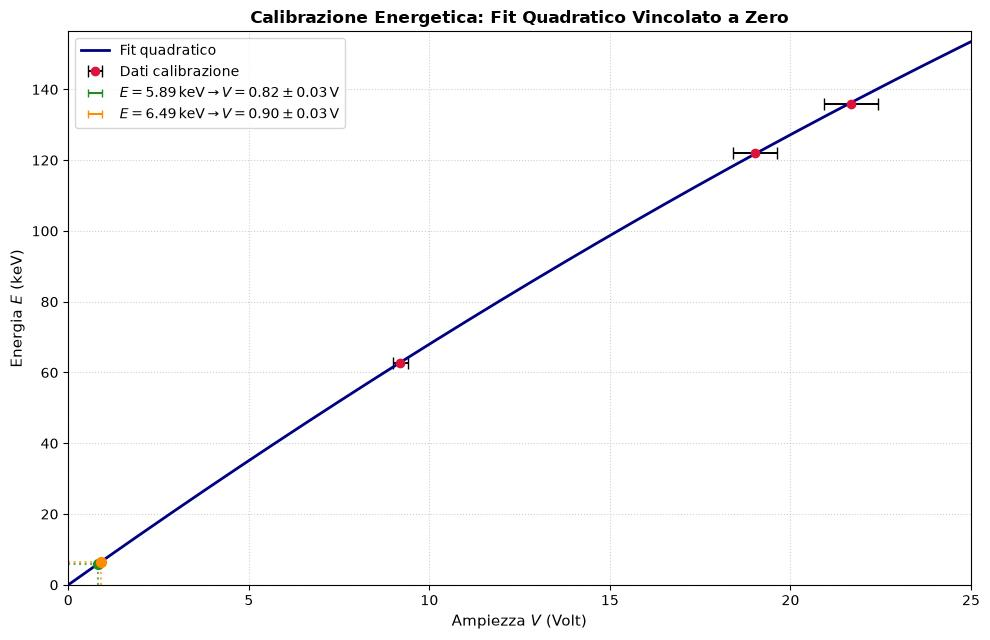
\includegraphics[width=0.88\textwidth]{figures/Calibrazione_fit_quadratico.jpeg}
    \caption{Curva di calibrazione energetica quadratica vincolata all'origine, costruita a partire dai tre picchi ad alta energia del $^{57}\text{Co}$. I punti evidenziati a bassa tensione illustrano l'estrapolazione a ritroso per le righe $K_\alpha$ e $K_\beta$ del $^{55}\text{Fe}$.}
    \label{fig:Calibrazione_fit_quadratico}
\end{figure}

Per validare la risposta del calorimetro nella regione sub-keV e a pochi keV, la funzione di calibrazione è stata invertita analiticamente per calcolare la posizione in tensione attesa per i fotoni caratteristici del $^{55}\text{Fe}$:
\begin{align}
    E = 5.89\,\text{keV} \quad &\Longrightarrow \quad V_{\text{att}} = 0.82 \pm 0.03\,\text{V}, \\
    E = 6.49\,\text{keV} \quad &\Longrightarrow \quad V_{\text{att}} = 0.90 \pm 0.03\,\text{V}.
\end{align}
Confrontando tali valori con le ampiezze misurate sperimentalmente sui fotopicchi non saturi del Ferro ($V_{\text{oss}} = 0.862\,\text{V}$ e $0.941\,\text{V}$), si riscontra un accordo entro le barre d'errore a circa $1.5\sigma$. La discrepanza relativa percentuale:
\begin{equation}
    \Delta_{\text{rel}} = \frac{|V_{\text{oss}} - V_{\text{att}}|}{V_{\text{oss}}}
\end{equation}
si attesta al $4.8\%$ per la riga da $5.89\,\text{keV}$ e al $4.6\%$ per la riga da $6.49\,\text{keV}$. L'accordo inferiore al $5\%$ su un'estrapolazione condotta lungo oltre un ordine di grandezza in tensione convalida sperimentalmente la solidità dell'approccio metodologico adottato.

\section{Calibrazione a Bassa Soglia Mediante Rinculi Nucleari}
\label{sec:calibrazione_rinculi_nucleari}

Nonostante l'eccellente coerenza riscontrata tra le righe del $^{57}\text{Co}$ e del $^{55}\text{Fe}$, la calibrazione energetica convenzionale presenta un limite intrinseco per la fisica della materia oscura: essa si basa interamente su \textit{rinculi elettronici} ($e^-/\gamma$), mentre l'interazione attesa per particelle massive WIMP avviene mediante \textit{rinculi nucleari}. 
A differenza di un rinculo elettronico, un rinculo nucleare tramette una frazione dell'energia cinetica ceduta al reticolo cristallino in difetti stabili. Tuttavia, come evidenziato in \cite{Angloher:2023_neutron_peak}, con le attuali incertezze non possiamo confermare se questa differenza esiste o meno, tuttavia se esiste è inferiore al 5\%.

Per ancorare direttamente la risposta del rivelatore nella regione di bassa soglia, la collaborazione CRESST ha recentemente validato un metodo di calibrazione basato sulla cattura radiativa di neutroni termici \cite{Angloher:2023_neutron_peak}. 

Nel setup sperimentale ai Laboratori Nazionali del Gran Sasso, il rivelatore è stato esposto a una sorgente neutronica di Americio-Berillio. I neutroni veloci emessi vengono moderati dalle schermature di polietilene, piombo e rame, raggiungendo il cristallo di $\text{CaWO}_4$ con energie termiche ($E_n \lesssim 25\,\text{meV}$). Tra i vari isotopi presenti, il $^{182}\text{W}$ presenta una sezione d'urto di cattura termica rilevante ($\sigma \approx 20.3\,\text{b}$), per poi diseccitarsi tramite emissione di un fotone $\gamma$ verso lo stato fondamentale del $^{183}\text{W}$ ($Q = 6190.7\,\text{keV}$):
\begin{equation}
    n + \,^{182}\text{W} \;\longrightarrow\; ^{183}\text{W}^* \;\longrightarrow\; ^{183}\text{W} + \gamma.
\end{equation}
A causa dell'elevata energia, il fotone $\gamma$ attraversa il cristallo senza interagire. Per conservazione del momento, il nucleo figlio di $^{183}\text{W}$ subisce un rinculo monoenergetico determinato da :
\begin{equation}
    E_R = \frac{E_\gamma^2}{2 M c^2} = 112.4\,\text{eV}.
\end{equation}
Questo processo genera un picco monoenergetico isolato a $112.4\,\text{eV}$ nel canale fononico, offrendo un punto di calibrazione ideale a rinculo nucleare puro.

Per determinare l'ampiezza equivalente a cui è atteso tale segnale sul nostro calorimetro, è stato eseguito un fit polinomiale di terzo grado vincolato a passare per l'origine, esteso a tutti e 5 i punti fiduciali disponibili (i tre picchi linearizzati del $^{57}\text{Co}$ e le due righe misurate del $^{55}\text{Fe}$):
\begin{equation}
    E(V) = a \cdot V^3 + b \cdot V^2 + c \cdot V.
\end{equation}
I parametri ottimali risultanti dal fit globale (riportato in Figura~\ref{fig:riga112eV}) sono:
\begin{align}
    a &= (-2.56 \pm 1.56) \times 10^{-3}\,\text{keV/V}^3, \\
    b &= (2.89 \pm 3.25) \times 10^{-2}\,\text{keV/V}^2, \\
    c &= (6.82 \pm 0.03)\,\text{keV/V}.
\end{align}

\begin{figure}[htbp]
    \centering
    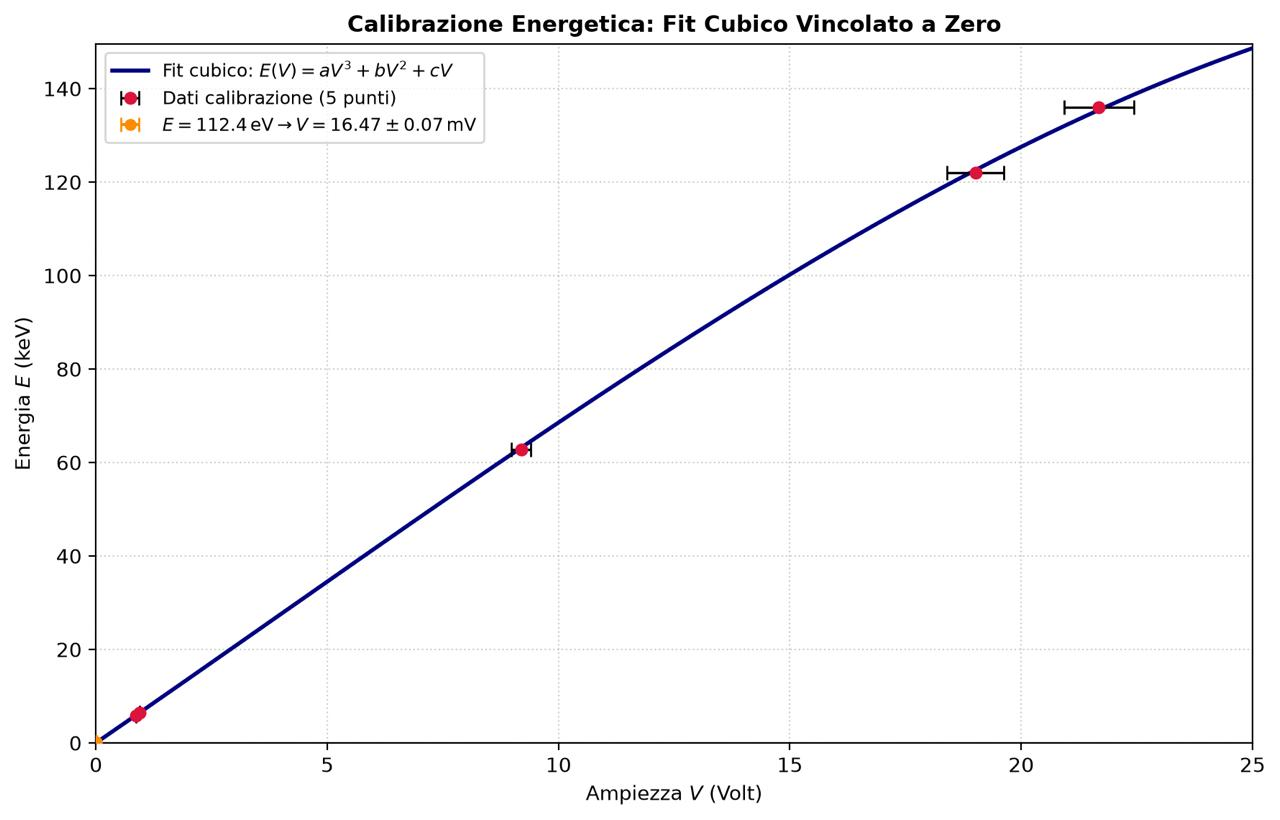
\includegraphics[width=0.88\textwidth]{figures/riga112eV.jpeg}
    \caption{Curva di calibrazione polinomiale di terzo grado vincolata all'origine, ottenuta combinando tutti e 5 i picchi sperimentali ($^{57}\text{Co}$ e $^{55}\text{Fe}$). Il punto in arancione individua l'ampiezza predetta per il rinculo nucleare da $112.4\,\text{eV}$ ($V = 16.47 \pm 0.07\,\text{mV}$).}
    \label{fig:riga112eV}
\end{figure}

Valutando la funzione invertita all'energia del rinculo nucleare ($E = 112.4\,\text{eV}$), si ricava la tensione attesa sul sensore:
\begin{equation}
    V(112.4\,\text{eV}) = 16.47 \pm 0.07\,\text{mV}.
\end{equation}
Come emerge chiaramente da Figura~\ref{fig:riga112eV}, la funzione si mantiene rigorosamente lineare lungo l'intera finestra sub-keV, con una pendenza determinata dal termine di primo grado ($c \approx 6.82\,\text{keV/V}$). La curvatura negativa diviene apprezzabile unicamente a tensioni elevate, ben al di sopra dell'escape peak da $62.8\,\text{keV}$. 

Questo riscontro certifica che, nella finestra a bassa soglia deputata all'osservazione dei candidati di materia oscura, il calorimetro risponde in modo lineare come ipotizzato inizialmente.